% Dieses Dokument muss mit PDFLatex geestzt werden
% Vorteil: Grafiken koennen als jpg, png, ... verwendet werden
%          und die Links im Dokument sind auch gleich richtig
%
%Ermöglicht \\ bei der Titelseite (z.B. bei supervisor)
%Siehe https://github.com/latextemplates/uni-stuttgart-cs-cover/issues/4
\RequirePackage{kvoptions-patch}
%
\documentclass[
               paper=a4,
%               twoside, % fuer die Betrachtung am Schirm ungeschickt
% Optionen fuer typearea.
               BCOR1.92mm,DIV12,headinclude, %je höher der DIV-Wert, desto mehr geht auf eine Seite - Hack für BCOR. Bei BCOR2mm sind die Fuellpunkte beim Inhaltsverzeichnis falsch
%               titlepage,
               bibliography=totoc,
%               idxtotoc,   %Index ins Inhaltsverzeichnis
%				liststotoc, %List of X ins Inhaltsverzeichnis, mit liststotocnumbered werden die Abbildungsverzeichnisse nummeriert
               headsepline,
               cleardoublepage=empty,
               parskip=half,
				pointlessnumbers, %f"ur englische Texte, dann unten \ifdeutsch und \ifenglisch anpassen.
%               draft    % um zu sehen, wo noch nachgebessert werden muss - wichtig, da Bindungskorrektur mit drin
               final   % ACHTUNG! - in pagestyle.tex noch Seitenstil anpassen
               ]{scrbook}

%Englisch:			   
\let\ifdeutsch\iffalse
\let\ifenglisch\iftrue

%Deutsch:
%\let\ifdeutsch\iftrue
%\let\ifenglisch\iffalse

			   
%%%
% Beschreibung:
% In dieser Datei werden zuerst die benoetigten Pakete eingebunden und
% danach diverse Optionen gesetzt. Achtung Reihenfolge ist entscheidend!
%
%%%


%%%
% Styleguide:
%
% Ein sehr kleiner Styleguide. Packages werden in Blöcken organisiert.
% Ein Block beginnt mit drei % in einer Zeile, dann % <Blocküberschrift>, dann 
% eine Liste der möglichen Optionen und deren Einstellungen, Gründe und Kommentare
% eine % Zeile in der sonst nichts steht und dann wieder %%% in einer Zeile.
%
% Zwischen zwei Blöcken sind 2 Leerzeilen!
% Zu jedem Paket werden soviele Optionen wie möglich/nötig angegeben
%
%%%

%%%
% Codierung
% Wir sind im 21 Jahrhundert, utf-8 löst so viele Probleme.
%
% Mit UTF-8 funktionieren folgende Pakete nicht mehr. Bitte beachten!
%   * fancyvrb mit § 
%   * easylist -> http://www.ctan.org/tex-archive/macros/latex/contrib/easylist/ 
\usepackage[utf8]{inputenc}
%
%%%

%%%
%Parallelbetrieb tex4ht und pdflatex
\makeatletter
\@ifpackageloaded{tex4ht}{\def\iftex4ht{\iftrue}}
                         {\def\iftex4ht{\iffalse}}
\makeatother
%%%


%%%
%Farbdefinitionen
\usepackage[hyperref,dvipsnames]{xcolor}
%


%%%
% Neue deutsche Rechtschreibung und Literatur statt "Literature", Nachfolger von ngerman.sty
\ifdeutsch
\usepackage[ngerman]{babel}
  %Ein "abstract" ist eine "Kurzfassung", keine "Zusammenfassung"
  \addto\captionsngerman{%
    \renewcommand\abstractname{Kurzfassung}%
  }
\else
%
%
% if you are writing in english
% für englische Texte, Hinweise zu weiteren, notwendigen Umstellungen in README.txt beachten
\usepackage[american]{babel}
\fi
%
%%%

%%%
% Anführungszeichen
% Zitate in \enquote{...} setzen, dann werden automatisch die richtigen Anführungszeichen verwendet.
\usepackage{csquotes}
%%%


%%%
% erweitertes Enumerate
\usepackage{paralist}
%
%%%


%%%
% fancyheadings (nicht nur) fuer koma
\usepackage[automark]{scrpage2} 
%
%%%


%%%
%Mathematik
%
\usepackage[fleqn,leqno]{amsmath} % Viele Mathematik-Sachen: Doku: /usr/share/doc/texmf/latex/amsmath/amsldoc.dvi.gz
%fleqn (=Gleichungen linksbündig platzieren) funktioniert nicht direkt. Es muss noch ein Patch gemacht werden:
\addtolength\mathindent{1em}%work-around ams-math problem with align and 9 -> 10
\usepackage{mathtools} %fixes bugs in AMS math
%
%for theorems, replacement for amsthm
\usepackage[amsmath,hyperref]{ntheorem}
\theorempreskipamount 2ex plus1ex minus0.5ex
\theorempostskipamount 2ex plus1ex minus0.5ex
\theoremstyle{break}
\newtheorem{definition}{Definition}[section]
%
%%%


%%%
% Intelligentes Leerzeichen um hinter Abkürzungen die richtigen Abstände zu erhalten, auch leere.
% siehe commands.tex \gq{}
\usepackage{xspace}
%Macht \xspace und \enquote kompatibel
\makeatletter
\xspaceaddexceptions{\grqq \grq \csq@qclose@i \} }
\makeatother
%
%%%


%%%
% Anhang
\usepackage{appendix}
%[toc,page,title,header]
%
%%%


%%%
% Grafikeinbindungen
\usepackage{graphicx}%Parameter "pdftex" unnoetig
\graphicspath{{\getgraphicspath}}
\newcommand{\getgraphicspath}{graphics/}
%
%%%


%%%
% Enables inclusion of SVG graphics - 1:1 approach
% This is NOT the approach of http://www.ctan.org/tex-archive/info/svg-inkscape,
% which allows text in SVG to be typeset using LaTeX
% We just include the SVG as is
\usepackage{epstopdf}
\epstopdfDeclareGraphicsRule{.svg}{pdf}{.pdf}{%
  inkscape -z -D --file=#1 --export-pdf=\OutputFile
}
%
%%%


%%%
% Enables inclusion of SVG graphics - text-rendered-with-LaTeX-approach
% This is the approach of http://www.ctan.org/tex-archive/info/svg-inkscape,
\newcommand{\executeiffilenewer}[3]{%
\IfFileExists{#2}
{
%\message{file #2 exists}
\ifnum\pdfstrcmp{\pdffilemoddate{#1}}%
{\pdffilemoddate{#2}}>0%
{\immediate\write18{#3}}
\else
{%\message{file up to date #2}
}
\fi%
}{
%\message{file #2 doesn't exist}
%\message{argument: #3}
%\immediate\write18{echo "test" > xoutput.txt}
\immediate\write18{#3}
}
}
\newcommand{\includesvg}[1]{%
\executeiffilenewer{#1.svg}{#1.pdf}%
{
inkscape -z -D --file=\getgraphicspath#1.svg %
--export-pdf=\getgraphicspath#1.pdf --export-latex}%
\input{\getgraphicspath#1.pdf_tex}%
}
%%%

%%%
% Tabellenerweiterungen
\usepackage{array} %increases tex's buffer size and enables ``>'' in tablespecs
\usepackage{longtable}
%
%%%

%%%
% Eine Zelle, die sich über mehrere Zeilen erstreckt.
% Siehe Beispieltabelle in Kapitel 2
\usepackage{multirow}
%
%%%


%%%
% Links verhalten sich so, wie sie sollen
\usepackage{url}
%
%%%


%%%
% Index über Begriffe, Abkürzungen
%\usepackage{makeidx} makeidx ist out -> http://xindy.sf.net verwenden
%
%%%

%%%
%lustiger Hack fuer das Abkuerzungsverzeichnis
%nach latex durchlauf folgendes ausfuehren
%makeindex ausarbeitung.nlo -s nomencl.ist -o ausarbeitung.nls 
%danach nochmal latex
%\usepackage{nomencl}
%	\let\abk\nomenclature %Deutsche Ueberschrift setzen
%	  	\renewcommand{\nomname}{List of Abbreviations}
%		%Punkte zw. Abkuerzung und Erklaerung
%	  	\setlength{\nomlabelwidth}{.2\hsize}
%	  	\renewcommand{\nomlabel}[1]{#1 \dotfill}
%		%Zeilenabstaende verkleinern
%	  	\setlength{\nomitemsep}{-\parsep}
%	\makenomenclature
%
%%%

%%%
% Logik für Tex
\usepackage{ifthen} %fuer if-then-else @ commands.tex
%
%%%


%%%
% unterschiedliche Fancy-Chapter-Styles
%\usepackage[Bjarne]{fncychap}
%\usepackage[Lenny]{fncychap}
%
%%%


%%%
%
\usepackage{listings}
%
%%%


%%%
%Alternative zu Listings ist fancyvrb. Kann auch beides gleichzeitig benutzt werden.
\usepackage{fancyvrb}
%\fvset{fontsize=\small} %Groesse fuer den Fliesstext. Falls deaktiviert: \normalsize
%Funktioniert mit UTF-8 nicht mehr
%\DefineShortVerb{\§} %Somit kann im Text ganz einfach |verbatim| text gesetzt werden.
\RecustomVerbatimEnvironment{Verbatim}{Verbatim}{fontsize=\footnotesize}
\RecustomVerbatimCommand{\VerbatimInput}{VerbatimInput}{fontsize=\footnotesize}
%
%%%


%%%
% Bildunterschriften bei floats genauso formatieren wie bei Listings
% Anpassung wird unten bei den newfloat-Deklarationen vorgenommen
% Caption2 vielleicht besser
\usepackage{caption}
%
%%%


%%%
% Ermoeglicht es, Abbildungen um 90 Grad zu drehen
% Alternatives Paket: rotating Allerdings wird hier nur das Bild gedreht, während bei lscape auch die PDF-Seite gedreht wird. 
%Das Paket lscape dreht die Seite auch nicht 
\usepackage{pdflscape}
%
%%%


%%%
% Fuer listings
% Wird für fancyvrb und für lstlistings verwendet
\usepackage{float}

%\usepackage{floatrow}
%% zustäzlich für den Paramter [H] = Floats WIRKLICH da wo sie deklariert wurden paltzieren - ganz ohne Kompromisse
% floatrow ist der Nachfolger von float
% Allerdings macht floatrow in manchen Konstellationen Probleme. Deshalb ist das Paket deaktiviert.
%
%%%


%%%
% Fuer Abbildungen innerhalb von Abbildungen
% Ersetzt das Paket subfigure
%\usepackage{subfig}
%
%%%


%%%
%Fuer Tabellen mit Variablen Spaltenbreiten
%\usepackage{tabularx}
%\usepackage{tabulary}
%
%%%


%%%
% Fußnoten
% 
%\usepackage{dblfnote}  %Zweispaltige Fußnoten
%
% Keine hochgestellten Ziffern in der Fußnote (KOMA-Script-spezifisch):
%\deffootnote[1.5em]{0pt}{1em}{\makebox[1.5em][l]{\bfseries\thefootnotemark}} 
%
% Abstand zwischen Fußnoten vergrößern:
%\setlength{\footnotesep}{.85\baselineskip}
%
%
\renewcommand{\footnoterule}{}             % Keine Trennlinie zur Fußnote 
\addtolength{\skip\footins}{\baselineskip} % Abstand Text <-> Fußnote
% Fußnoten immer ganz unten auf einer \raggedbottom-Seite
\usepackage{fnpos}
%
%%%


%%%
%
\raggedbottom     % Variable Seitenhöhen zulassen
%
%%%


%%%
% Falls die Seitenzahl bei einer Referenz auf eine Abbildung nur dann angegeben werden soll,
% falls sich die Abbildung nicht auf der selben Seite befindet...
\iftex4ht
%tex4ht does not work well with vref, therefore we emulate vref behavior
\newcommand{\vref}[1]{\ref{#1}}
\else
\ifdeutsch
\usepackage[ngerman]{varioref}
\else
\usepackage{varioref}
\fi
\fi
%%%

%%%
% Noch schoenere Tabellen als mit booktabs mit http://www.zvisionwelt.de/downloads.html
\usepackage{booktabs} 
%
%\usepackage[section]{placeins}
%
%%%


%%%
%Fuer Graphiken. Allerdings funktioniert es nicht zusammen mit pdflatex
%\usepackage{gastex} % \tolarance kann dann nicht mehr umdefiniert werden
%
%%%


%%%
%
%\usepackage{multicol}
%\usepackage{setspace} % kollidiert mit diplomarbeit.sty
%
%http://www.tex.ac.uk/cgi-bin/texfaq2html?label=floats
%\usepackage{flafter} %floats IMMER nach ihrer Deklaration platzieren
%
%%%


%%%
%schoene TODOs
\usepackage{todonotes}
\let\xtodo\todo
\renewcommand{\todo}[1]{\xtodo[inline,color=black!5]{#1}}
\newcommand{\utodo}[1]{\xtodo[inline,color=green!5]{#1}}
\newcommand{\itodo}[1]{\xtodo[inline]{#1}}
%
%%%


%%%
% Neue Pakete bitte VOR hyperref einbinden. Insbesondere bei Verwendung des
% Pakets "index" wichtig, da sonst die Referenzierung nicht funktioniert.
% Für die Indizierung selbst ist unter http://xindy.sourceforge.net
% ein gutes Tool zu erhalten 
%%%


%%%
%
% hier also neue packages einbinden
%
%%%


%%%
% ggf.in der Endversion komplett rausnehmen. dann auch \href in commands.tex aktivieren
% Alle Optionen nach \hypersetup verschoben, sonst crash
%
\usepackage[]{hyperref}%siehe auch: "Praktisches LaTeX" - www.itp.uni-hannover.de/~kreutzm
%
%% Da es mit KOMA 3 und xcolor zu Problemen mit den global Options kommt MÜSSEN die Optionen so gesetzt werden.
%

% Eigene Farbdefinitionen ohne die Namen des xcolor packages
\definecolor{darkblue}{rgb}{0,0,.5}
\definecolor{black}{rgb}{0,0,0}

\hypersetup{
	breaklinks=true,
	bookmarksnumbered=true,
	bookmarksopen=true,
	bookmarksopenlevel=1,
	breaklinks=true,
	colorlinks=true,
	pdfstartview=Fit,
	pdfpagelayout=SinglePage,
	%
	filecolor=darkblue,
	urlcolor=darkblue,
	linkcolor=black,
	citecolor=black
}
%
%%%


%%%
% cleveref für cref statt autoref, da cleveref auch bei Definitionen funktioniert
\ifdeutsch
\usepackage[ngerman,capitalise,nameinlink]{cleveref}
\else
\usepackage[capitalise,nameinlink]{cleveref}
\fi
%%%


%%%
% Zur Darstellung von Algorithmen
% Algorithm muss nach hyperref geladen werden
\usepackage[chapter]{algorithm} 
\usepackage[]{algpseudocode}
%
%%%


%%%
% Schriften
\input{preambel/fonts}
%
%%%


%%%
% Links auf Gleitumgebungen springen nicht zur Beschriftung,
% Doc: http://mirror.ctan.org/tex-archive/macros/latex/contrib/oberdiek/hypcap.pdf
% sondern zum Anfang der Gleitumgebung
\usepackage[all]{hypcap}
%%%


%%%
% Deckblattstyle
%
% für englische Ausarbeitungen "language=english" benutzen
\usepackage[
	title={Distributed Data Analytics Using Graph Processing Frameworks},
	author={Chen Li},
	type={Master thesis},
	institute=ipvs,
	number=0202-0006,
	course={INFOTECH},
	examiner={Prof.\ Dr.\ rer.\ nat.\ Dr.\ h.\ c.\ Kurt Rothermel},
	supervisor={Dr.\ rer.\ nat.\ Muhammad Adnan Tariq,\\Dipl.-Inf.\ Christian Mayer},
	startdate={June 22, 2015}, % English: July 5, 2013;    ISO: 2013-07-05
	enddate={December 22, 2015}, % English: January 5, 2014; ISO: 2014-01-05
	crk={G.2.2, I.6},
	%language=german
	language=english
	]{uni-stuttgart-cs-cover}
%
%%%


%%%
%Bugfixes packages
%\usepackage{fixltx2e} %Fuer neueste LaTeX-Installationen nicht mehr benoetigt - bereinigte einige Ungereimtheiten, die auf Grund von Rueckwaertskompatibilitaet beibahlten wurden.
%\usepackage{mparhack} %Fixt die Position von marginpars (die in DAs selten bis gar nicht gebraucht werden}
%\usepackage{ellipsis} %Fixt die Abstaende vor \ldots. Wird wohl auch nicht benoetigt.
%
%%%


%%%
% Rand
\input{preambel/margins}
%
%%%


%%%
% Optionen                                                                  
%
%Skip=0 funktioniert nicht
\captionsetup{format=hang,labelfont=bf,justification=justified,singlelinecheck=false,skip=0pt}
%
%neue float Umgebung fuer Listings, die mittels fancyvrb gesetzt werden sollen
\floatstyle{ruled}
\newfloat{Listing}{tbp}{code}[chapter]
\newfloat{Algorithmus}{tbp}{alg}[chapter]
%
%amsmath
%\numberwithin{equation}{section}
%\renewcommand{\theequation}{\thesection.\Roman{equation}}
%
%pdftex
\pdfcompresslevel=9
%
%Tabellen (array.sty)
\setlength{\extrarowheight}{1pt}
%
%
\input{preambel/chapterheads}
%
%%%


%%%
%Minitoc-Einstellungen
%\dominitoc
%\renewcommand{\mtctitle}{Inhaltsverzeichnis dieses Kapitels}
%
% Disable single lines at the start of a paragraph (Schusterjungen)
\clubpenalty = 10000
%
% Disable single lines at the end of a paragraph (Hurenkinder)
\widowpenalty = 10000 \displaywidowpenalty = 10000
%
%http://groups.google.de/group/de.comp.text.tex/browse_thread/thread/f97da71d90442816/f5da290593fd647e?lnk=st&q=tolerance+emergencystretch&rnum=5&hl=de#f5da290593fd647e
%Mehr Infos unter http://www.tex.ac.uk/cgi-bin/texfaq2html?label=overfull
\tolerance=2000
\setlength{\emergencystretch}{3pt}   % kann man evtl. auf 20 erhoehen
\setlength{\hfuzz}{1pt}
%
%%%


%%%
% Fuer listings.sty
\lstset{language=XML,
        showstringspaces=false,
        extendedchars=true,
        basicstyle=\footnotesize\ttfamily,
        commentstyle=\slshape,
        stringstyle=\ttfamily, %Original: \rmfamily, damit werden die Strings im Quellcode hervorgehoben		zusaetzlich evtl.: \scshape oder \rmfamily durch \ttfamily ersetzen. Dann sieht's aus, wie bei fancyvrb
        breaklines=true,
        breakatwhitespace=true,
        columns=flexible,
        aboveskip=0mm, %deaktivieren, falls man lstlistings direkt als floating object benutzt (\begin{lstlisting}[float,...])
        belowskip=0mm, %deaktivieren, falls man lstlistings direkt als floating object benutzt (\begin{lstlisting}[float,...])
        captionpos=b
}
\ifdeutsch
\renewcommand{\lstlistlistingname}{Verzeichnis der Listings}
\fi
%
%%%


%%%
%fuer algorithm.sty: - falls Deutsch und nicht Englisch. Falls Englisch als Sprache gewählt wurde, bitte die folgenden beiden Zeilen auskommentieren.
%\floatname{algorithm}{Algorithmus}
\ifdeutsch
\renewcommand{\listalgorithmname}{Verzeichnis der Algorithmen}
\fi
%
%%%


%%%
% Das Euro Zeichen 
% Fuer Palatino (mathpazo.sty): richtiges Euro-Zeichen
% Alternative: \usepackage{eurosym}
\newcommand{\EUR}{\ppleuro}
%
%%%


%%%
%
% Float-placements - http://dcwww.camd.dtu.dk/~schiotz/comp/LatexTips/LatexTips.html#figplacement
% and http://people.cs.uu.nl/piet/floats/node1.html
\renewcommand{\topfraction}{0.85}
\renewcommand{\bottomfraction}{0.95}
\renewcommand{\textfraction}{0.1}
\renewcommand{\floatpagefraction}{0.75}
%\setcounter{totalnumber}{5}
%
%%%

%%%
%
% Bei Gleichungen nur dann die Nummer zeigen, wenn die Gleichung auch referenziert wird
%
% Funktioniert mit MiKTeX Stand 2012-01-13 nicht. Deshalb ist dieser Schalter deaktiviert.
%
%\mathtoolsset{showonlyrefs}
%
%%%

%%%
%Optischer Randausgleich
\usepackage{microtype}
%%%

%%%
% Rueckverweise aus dem Literaturverzeichnis
\usepackage[hyperpageref]{backref}
\ifdeutsch
% Deutscher Text
\newcommand{\babelbackrefnotcited}{\relax}
\newcommand{\babelbackrefcitedsingle}[1]{(Zitiert auf Seite~#1)}
\newcommand{\babelbackrefcitedmulti}[1]{(Zitiert auf den Seiten~#1)}
\newcommand{\babelbackrefand}{und}
\else
% Englischer Text
\newcommand{\babelbackrefnotcited}{\relax}
\newcommand{\babelbackrefcitedsingle}[1]{(Cited on page~#1)}
\newcommand{\babelbackrefcitedmulti}[1]{(Cited on pages~#1)}
\newcommand{\babelbackrefand}{and}
\fi
% Tweak backref
\renewcommand{\backreftwosep}{ \babelbackrefand~} % seperate 2 pages
\renewcommand{\backreflastsep}{ \babelbackrefand~} % seperate last of longer list
\renewcommand*{\backref}[1]{} % Standard deaktivieren
\renewcommand*{\backrefalt}[4]{% 
\ifcase #1 %
\babelbackrefnotcited%
\or
\babelbackrefcitedsingle{#2}%
\else
\babelbackrefcitedmulti{#2}%
\fi}
%
%%%


 %Der untere Rand darf "flattern"
\raggedbottom

%%%
% Wie tief wird das Inhaltsverzeichnis aufgeschlüsselt
% 0 --\chapter
% 1 --\section % fuer kuerzeres Inhaltsverzeichnis verwenden - oder minitoc benutzen
% 2 --\subsection
% 3 --\subsubsection
% 4 --\paragraph
\setcounter{tocdepth}{1}
%
%%%

\makeindex

%Angaben in die PDF-Infos uebernehmen
\makeatletter
\hypersetup{
            pdftitle={}, %Titel der Arbeit
            pdfauthor={}, %Author
            pdfkeywords={}, % CR-Klassifikation und ggf. weitere Stichworte
            pdfsubject={}
}
\makeatother

\begin{document}
%tex4ht-Konvertierung verschönern
\iftex4ht
% tell tex4ht to create picures also for formulas starting with '$'
% WARNING: a tex4ht run now takes forever!
\Configure{$}{\PicMath}{\EndPicMath}{} 
%$ % <- syntax highlighting fix for emacs
\Css{body {text-align:justify;}}

%conversion of .pdf to .png
\Configure{graphics*}  
         {pdf}  
         {\Needs{"convert \csname Gin@base\endcsname.pdf  
                               \csname Gin@base\endcsname.png"}%  
          \Picture[pict]{\csname Gin@base\endcsname.png}%  
         }  
\fi

%Tipp von http://goemonx.blogspot.de/2012/01/pdflatex-ligaturen-und-copynpaste.html
%siehe auch http://tex.stackexchange.com/questions/4397/make-ligatures-in-linux-libertine-copyable-and-searchable
%
%ONLY WORKS ON MiKTeX
%On other systems, download glyphtounicode.tex from http://pdftex.sarovar.org/misc/
%
\input glyphtounicode.tex
\pdfgentounicode=1

\VerbatimFootnotes %verbatim text in Fußnoten erlauben. Geht normalerweise nicht.
%\frontmatter
\input{macros/commands}
\pagenumbering{arabic}
\Titelblatt

%Eigener Seitenstil fuer die Kurzfassung und das Inhaltsverzeichnis
\deftripstyle{preamble}{}{}{}{}{}{\pagemark}
%Doku zu deftripstyle: scrguide.pdf
\pagestyle{preamble}
\renewcommand*{\chapterpagestyle}{preamble}

%Kurzfassung / abstract
%auch im Stil vom Inhaltsverzeichnis
\ifdeutsch
\section*{Kurzfassung}
\else
\section*{Abstract}
\fi

In recent years, with the growth of graphs size and associated data, e.g. Facebook user graph, large graphs trend to be distributed and processed in parallel on the cluster by using graph processing frameworks such as Pregel and PowerGraph. Graph processing frameworks generally provide a vertex-centric programming model. However, some important problems do not have available algorithms in this model. This thesis presents novel algorithms in vertex-centric programming paradigm for two problems: distributed subgraph isomorphism, and geospatial simulation using Agent-Based Cellular Automata. We evaluate the proposed algorithms on PowerGraph, and use these algorithms to examine a framework prototype called GrapH with respect to the improvement in communication.
%We evaluate the proposed algorithms on PowerGraph and show that heterogeneity of the vertex synchronization costs leads to communication imbalance. These algorithms are also used to examine the communication improvement of a framework prototype called GrapH, which takes the heterogeneity into account and introduces adaptive partitioning during the execution.

The subgraph isomorphism problem is to determine whether a given graph contains any subgraph that is isomorphic to a given pattern.
%, which is well known as NP-complete problem and is fundamental for many applications such as analysis of social networks and substructure search in chemistry. 
Most existing algorithms for subgraph isomorphism are highly computation intensive and are not capable to scale to large graphs. As solving subgraph isomorphism often requires a global overview of graph, developing a vertex-centric algorithm is very challenging. We present a distributed algorithm (DSI) and two variants (optimized DSI and PDSI) based on the GAS model for subgraph isomorphism. We also analyse the properties of the algorithms and point out the bottlenecks for the performance.

Geospatial simulation has assisted the investigation and modelling the environmental systems, which helps people understanding complex dynamics of our society and making better decisions. As the scale of simulations becomes larger, simulation trends to be executed on distributed systems. Therefore using graph processing frameworks is a good option for simulation. Thus we present an algorithm for geospatial simulation using Agent-Based Cellular Automata.

Our evaluation show that optimized DSI needs on average only one third of the execution time as DSI needs. PDSI can remarkably reduce the runtime with a low proportion, and still be able to find a relative reasonable quantity of the isomorphic subgraphs. Moreover, algorithms for both subgraph isomorphism and geospatial simulation display heterogeneous vertex synchronization costs. Finally, we show that by taking the heterogeneity into account and introducing adaptive partitioning GrapH reduces overall communication more than 20\%, compared with PowerGraph partitioning strategy.

%Besides evaluation of the proposed algorithms on PowerGraph, this thesis also shows that heterogeneity of the vertex synchronization costs leads to communication imbalance. The proposed algorithms were executed on a framework prototype under developing in University of Stuttgart, which takes the heterogeneity into account and introduces adaptive partitioning during the execution to reduce the communication between machines.

\cleardoublepage


% BEGIN: Verzeichnisse

\iftex4ht
\else
\microtypesetup{protrusion=false}
\fi

%%%
% Literaturverzeichnis ins TOC mit aufnehmen, aber nur wenn nichts anderes mehr hilft!
% \addcontentsline{toc}{chapter}{Literaturverzeichnis}
%
% oder zB
%\addcontentsline{toc}{section}{Abkürzungsverzeichnis}
%\section*{Abkürzungsverzeichnis}
%
%%%

%Inhaltsverzeichnis anlegen
\tableofcontents

% Bei einem ungünstigen Seitenumbruch im Inhaltsverzeichnis, kann dieser mit
% \addtocontents{toc}{\protect\newpage}
% an der passenden Stelle im Fließtext erzwungen werden.

%listof* untereinandergesetzt
%ACHTUNG! Falls ein anderer Kapitelstil gewählt wird, muss der Code hier evtl.
%  angepasst werden
\begingroup 
\makeatletter
  \def\@makeschapterhead#1{%
  \vspace*{10\p@}%
  {\parindent \z@ \raggedright \reset@font
            \normalfont \vphantom{\@chapapp{} \thechapter}
        \par\nobreak\vspace*{10\p@}%
        \interlinepenalty\@M
    {\huge \bfseries %
	%
	%Default-Schrift: Serifenhaft (fuer englische Dokumente)
	% Dann sowohl A als auch B deaktivieren
    %A) Fuer serifenlose Schrift folgende Zeile aktivieren:
	\ifdeutsch
    \fontfamily{phv}\selectfont
	\fi
	%B) Fuer Kapitaelchen folgende Zeile aktivieren:
	%\fontseries{m}\fontshape{sc}\selectfont
	%
	#1\par\nobreak}
    %\vspace*{1\p@}%
\makebox[\textwidth]{\hrulefill}%    \hrulefill alone does not work
    \par\nobreak
    \vskip 5\p@
  }}
\makeatother
\let\cleardoublepage\clearpage
\listoffigures
\let\cleardoublepage\relax
\listoftables

%Wird nur bei Verwendung von der lstlisting-Umgebung mit dem "caption"-Parameter benoetigt
%\lstlistoflistings 
%ansonsten:
\ifdeutsch
\listof{Listing}{Verzeichnis der Listings}
\else
\listof{Listing}{List of Listings}
\fi

%mittels \newfloat wurde die Algorithmus-Gleitumgebung definiert.
%Mit folgendem Befehl werden alle floats dieses Typs ausgegeben
\ifdeutsch
\listof{Algorithmus}{Verzeichnis der Algorithmen}
\else
\listof{Algorithmus}{List of Algorithms}
\fi
%\listofalgorithms %Ist nur für Algorithmen, die mittels \begin{algorithm} umschlossen werden, nötig

\endgroup

\cleardoublepage

\iftex4ht
\else
%Optischen Randausgleich und Grauwertkorrektur wieder aktivieren
\microtypesetup{protrusion=true}
\fi

% END: Verzeichnisse


\renewcommand*{\chapterpagestyle}{scrplain}
\pagestyle{scrheadings}
\input{preambel/pagestyle}
%
%
% ** Hier wird der Text eingebunden **
%
%\input{content/einleitung}
%\input{...weitere Kapitel...}
%\input{content/kapitel2}
\chapter{Introduction}\label{chap:c1}

As our society has entered the information age, more and more things are measured and recorded by the digital data, which is increasing extremely. Social network records our social behaviors, and mobile devices keep our personal data such as life experiences and mobility data. These large datasets are often referred as Big Data. The Big Data analytics increasingly attracts academia and industry to find feasible solutions for the challenges introduced by processing huge datasets. Large companies such as Google and Facebook spend more and more human and finance resources on Big Data, such as web, user or financial data, to mine valuable information.

Accurate data analysis can reveal hidden information and lead people to better decision making. However, the traditional data analysing applications are generally not adequate to handle such large datasets. Due to the computing limitation of single machine and the size and complexity of the data, a single machine is not capable to process Big Data. Cloud is more powerful in computation and therefore is usually a good option for Big Data analysis. The datasets are distributed over many computers and the computation on the data is executed in parallel, so that results could be delivered in a reasonable time. Distributed and parallel computation on large datasets required the user having expert knowledge in both distributed systems and algorithmic design in the past.

To obscure the complexity of the data distribution, computation parallelization and failure handling, Google initiated the MapReduce project in 2004\cite{dean2008mapreduce}, in which processes execute computation on data splits independently. However MapReduce programming model is inefficient to deal with the algorithms for processing graph data, since iterative computation over graph data requires MapReduce to save entire state of the graph form one stage to the next, which incurs communication and serialization overhead. 

In contrast to MapReduce, graph processing frameworks such as Pregel\cite{malewicz2010pregel} and PowerGraph\cite{gonzalez2012powergraph} keep states of the graph in memory and perform parallel iterative computation on the graph with fault tolerance. These frameworks partition large graph over machines, which is critical for the performance for these frameworks. A good partitioning should have balanced workload on each machine and balanced communication between machines. Early frameworks such as Pregel use edge-cut and randomly assign vertices to machines, which is an inefficient strategy, especially for natural graphs with power-law degree distribution. To overcome this challenge, PowerGraph improves partitioning by adopting vertex-cut and assigning edges to machines in a collaborated way. In vertex-cut, a vertex with higher degree is more likely to span over several machines, and communication is needed when synchronizing data of these spanning vertices. In this thesis, we denote the size of vertex data to be synchronized of spanning vertex as vertex synchronization costs. This strategy is based on an assumption that the vertex synchronization costs for each vertex (if it is spanned over machines) are homogeneous. However, for many algorithms, the vertex synchronization costs are heterogeneous. To better partition large graphs, more sophisticated strategies are desired. These frameworks provide a similar programming model in which users express their algorithms in a vertex-centric program that thinks as a vertex. In PowerGraph, this programming paradigm is summarized as GAS (\textbf{G}ather, \textbf{A}pply and \textbf{S}catter) model. Vertex-centric program of GAS model running on each vertex iteratively gathers information from its neighbors, updates its own data by using the gathered information and informs its neighbors again.

As graph processing frameworks can efficiently solve many graph-related problems by parallelism and the GAS programming paradigm is expressive, many important and popular graph algorithms have been redesigned in GAS model, such as PageRank and shortest paths. However, some important problems like subgraph isomorphism are still open, because the existing algorithms for those problem were not designed to think as a vertex.
Therefore we design algorithms on graph processing frameworks for two significant applications. 

The first one is subgraph isomorphism, which is fundamental for many problems such as clique problem. It is widely applied in diverse areas such as biochemistry, informatics and artificial intelligence. In cheminformatics, subgraph isomorphism is used to find similarities between chemical compounds from their structural formula. It has also been used in social network analysis. The subgraph isomorphism problem is a computational task with two graphs $G$ and $P$ as input, to determine whether $G$ contains subgraphs that are isomorphic to $P$. This problem is well-known as a NP-complete problem. However all existing algorithms for subgraph isomorphism do not fit to the programming model in graph processing frameworks. Because existing algorithms usually need a global overview to assist computation, while vertex-centric program only has access to local and adjacent data.

The second one is geospatial simulation. The geo-informatics with spatial and temporal data can assist the investigation and modelling the environmental systems. For example, traffic simulation helps transportation authorities to make good decisions to keep the transportation system working. As the scale of simulations becomes larger, simulations trend to be executed on distributed systems. Therefore, graph processing framework is a good option, as it can naturally simulate the geospatial informations.

In particular the contributes of this thesis are summarized as following:

	\begin{itemize}
	\item A novel algorithm (DSI) for subgraph isomorphism that fits to the GAS programming paradigm and analysis of the algorithm.
	\item The optimized DSI algorithm with two techniques and a variant algorithm called PDSI that balances the complexity and completeness. 
	\item An algorithm for geospatial simulation using Agent-Based Cellular Automata.
	\item Implementations of proposed algorithms on PowerGraph and GrapH.
	\item A comprehensive evaluation of the proposed algorithms on PowerGraph and evaluation of GrapH with the proposed algorithms with respect to the improvement of communication.
	\end{itemize}


\section*{Outline}

This thesis is organized as follows:
\begin{description}
\item[Chapter \ref{chap:c2} -- \nameref{chap:c2}:] introduces the background knowledge of graph processing frameworks and their pros and cons.
\item[Chapter \ref{chap:c3} -- \nameref{chap:c3}:] discusses the problem of graph pattern matching, and then gives an algorithm and its variants to solve the subgraph isomorphism problem in a distributed setting and analysis of the algorithms. 
\item[Chapter \ref{chap:c4} -- \nameref{chap:c4}:] shows that graph processing framework can be used for geospatial simulation and gives a simulation algorithm of Agent-Based Cellular Automata.
\item[Chapter \ref{chap:c5} -- \nameref{chap:c5}:] presents the evaluation environment, evaluation results and analysis of the proposed algorithms. We show the heterogeneity of the vertex synchronization costs, therefore we evaluate a framework prototype with the algorithms, which improves communication.
\item[Chapter \ref{chap:c6} -- \nameref{chap:c6}:] draws a conclusion and shows possible improvements for both frameworks and the presented algorithms.

\end{description}
\chapter{Graph Processing Framework}
\label{chap:c2}

The topic of Big Data has been attracting the attention in academia and industry. Extracting useful information hidden in large datasets can assist people to make better decisions. However, a single machine is often incapable to handle such large and complex datasets. Therefore the common solution is to distribute the data over the cloud and compute in parallel.

To separate distributed and parallel computation from data analytics, Google initiated MapReduce project. MapReduce offers a programming model and its associated implementation for processing large datasets\cite{dean2008mapreduce}. A MapReduce program consists of the function \emph{map} that takes an input key/value pairs and generates intermediate key/value pairs, and the function \emph{reduce} performs a merge operation on the intermediate results. It is implemented as a scalable and fault-tolerant interface. Users only need to specify the map and reduce functions, and the system executes these functions on the large datasets in a parallel fault-tolerant manner.

While the MapReduce abstraction is optimized for parallel computation on different splits of the data independently from each other, it is inefficient for graph algorithms. As MapReduce expresses a graph algorithm as a series of fine-granular MapReduce jobs, it has to pass the entire state of the graph from one stage to the next by writing data to the stable storage, which incurs much communication and serialization overhead. It also adds the programming complexity to the user. 

In addition, graph problems often exhibit the following properties that introduce challenges for efficient parallelism\cite{lumsdaine2007challenges}.

\begin{itemize}
	\item \textbf{Data-driven computations.} Computations of graph algorithms are often driven by the graph structure, while graph algorithms generally specify the computation on the vertices and edges of the graph. Therefore, parallel computation on different parts of the graph makes it difficult to partition the graph. 
	\item \textbf{Unstructured problems.} Data associated with the graph are unstructured in general, which challenge the parallelism based on partitioning the graph. Poorly partitioned graph limits the scalability and leads to workload imbalance. 
	\item \textbf{Poor locality.} Graphs describe the relationships between entities, which are often unstructured and irregular. Therefore data access shows poor locality, which limits the performance of a system.
	\item \textbf{High data access to computation ratio.} Graph algorithms often interest in exploring the information in a graph rather than computation intensive processing on graph data. Frequently data access with poor locality will result in long latency.
\end{itemize}

Graph analytics becomes increasingly important with trend of Big Data for solving many problems in widely range. In order to address the challenge of graph algorithms to MapReduce-based frameworks, researchers proposed graph processing frameworks such as Pregel\cite{malewicz2010pregel} and PowerGraph\cite{gonzalez2012powergraph}. These frameworks provide users with an interface to specify their algorithms in a vertex-centric program, in which each vertex generally gathers data from its neighbors, updates its own data and informs neighbors about the change. Frameworks distribute the graph over cluster, execute the vertex-centric program on each vertex in a parallel manner and provide fault-tolerant. In contrast to MapReduce, these frameworks keep states of the graph, i.e. vertices and edges, during the computation.

\section{Pregel}

Pregel is a scalable and fault-tolerant general-purpose platform on which large scale graphs can be processed in a distributed environment. The API provided by Pregel is sufficient to implement many graph algorithms over arbitrary graph representations, and hides the details of distribution, such as message passing and fault tolerance.

\subsection{Computation Model}

The input graph to Pregel is a directed graph. Each vertex has a unique identifier and is associated with mutable user-defined data. Each edge is associated to its source vertex and mutable user-defined data. As there are lots of file formats of graphs, Pregel allows user to define how to interpret an file to the input graph.

Pregel follows the Bulk Synchronous Parallel (BSP) model\cite{valiant1990bridging}, which defines the synchronous computation and communication. The computation in Pregel is associated with vertices, which consists of a sequence of iterations, namely \textit{superstep}. Initially all the vertices are activated by the framework, and all active vertices are involved in the computation in any given superstep. Within each superstep, each vertex in parallel receives the message sent to it in the last superstep and invokes the same user-defined vertex function. The vertex function specifies the behavior according to the graph algorithm at a single vertex in a superstep, which can modify the data associated with the vertex and send messages to other vertices. A vertex decides to halt and becomes inactive when there is no further work to do, but it can be reactivated externally by the messages from others. If a vertex is in the inactive state, the framework will not execute the vertex function in the next superstep. The program terminates when all vertices decide to halt and no message in transit.

A vertex can send messages directly to others, even if the target vertex is not a neighbor. The message consists of a user-defined value and the destination vertex. The messages sent in current superstep are guaranteed to be delivered in the next superstep and not duplicated. The vertex function in Pregel is even allowed to modify the topology of the graph.

When the destination vertex of a message is on another machine, communication overhead is incurred, which might be reduced in some cases. For example, in the PageRank algorithm, received floating valued messages are summed up and then used in the vertex function. The messages sent to a same vertex can be combined to one message to reduce the overhead, if the combination operation is commutative and associative. Because the sequence of performing combination operation does not effect the final result.

Pregel also provides \textit{aggregators} for statistics and global coordination. Each vertex can submit a value to an aggregator in a superstep, and the aggregator combines these values to a single one, which is available in the next superstep. For example, a serial of different computations are performed over supersteps, and an aggregator decides to move to next computation when all vertices have fulfilled some requirements.

The output of the framework is the data generated by the vertices. Generally it is the same directed graph as input, but some algorithms would add or remove vertices or edges during the computation.

\subsection{Pregel Achitecture}

Pregel was designed to run on the Google cluster architecture. Each cluster has thousands of PCs. Pregel divides a graph into partitions, each of which contains a set of vertices and their associating out-going edges. A random hash by default is applied to assign a vertex to a partition. This will affect the performance, as many algorithms can benefit from a heuristic partitioning.

Basically a Pregel program executes like following. Many copies of the program start on a cluster. One of these is chosen as the master, which only coordinates the execution. The others, namely workers, register themselves to the master. The master determines the partitions and assigns one or more partitions to each worker. Each worker loads a part of the graph assigned by the master, maintains the state of the graph, executes vertex function and manages sending and receiving messages. The master instructs the workers to perform a superstep and waits for the response from the workers.

Pregel implements fault tolerance by \textit{checkpointing}. The workers save their partitions to stable storage, including vertex data, edge data, and incoming messages, and the master saves the aggregator values. The master pings the workers to detect the failure of the workers. When a worker does not receive a ping from the master after a specified period, the worker terminates the execution. When the master does not receive the response from a worker, then it deem the worker failed. When any worker fails, the master assigns the partitions in the failed workers to other available workers. They reload the partitions from the previous checkpoint and repeat the missing computations to the current superstep.

%\subsection{Performance}

%Many applications of graph algorithms, like PageRank and Shortest Path, have been implemented on Pregel framework. The experiments with the single-source shortest paths (SSSP) show that Pregel has a satisfactory performance with relatively little coding effort and a better scaling performance comparing with others.

\section{GraphLab}

In \cite{Low+al:uai10graphlab} the researchers argue that many algorithms of Machine Learning and Data Mining are characterized by asynchronous, dynamic, graph-parallel computation. Distributed GraphLab in shared-memory setting is presented to provide a high-level distributed abstraction for those algorithms.

\subsection{Computation Model}

The computation model of GraphLab has three major parts, the data graph, the update function and the sync operation. The data graph is similar to the one in Pregel. In GraphLab the program state and user-defined data $D$ are directly stored in the data graph $G=(V,E,D)$. Users are allowed to associate any data with vertices $\{D_v: v \in V\}$ and edges $\{D_{u \leftrightarrow v}: \{u,v\} \in E\}$. It is important to notice that GraphLab does not distinguish the directions of edges. Although the graph data can be modified, the structure of the graph is not allowed to be changed during execution. 

The update function $f(v,S_v) \rightarrow (S_v, T)$, which is a synonym of the vertex function, takes the data within the scope $S_v$ of a vertex $v$ as input, and returns the updated data and the scheduled vertices $T$ for further execution. The scope of a vertex includes the vertex and its adjacent edges and vertices as well as the associated data, as shown in Figure~\ref{fig:Scope}. The dashed rectangle marks the scope of vertex 3. The update function on vertex 3 can read and write all data in $S_3$, which includes vertex data $D_2, D_3, D_4$ and edge data $D_{2 \leftrightarrow 3}, D_{3 \leftrightarrow 4}$.

\begin{figure}[H]
  \begin{center}
    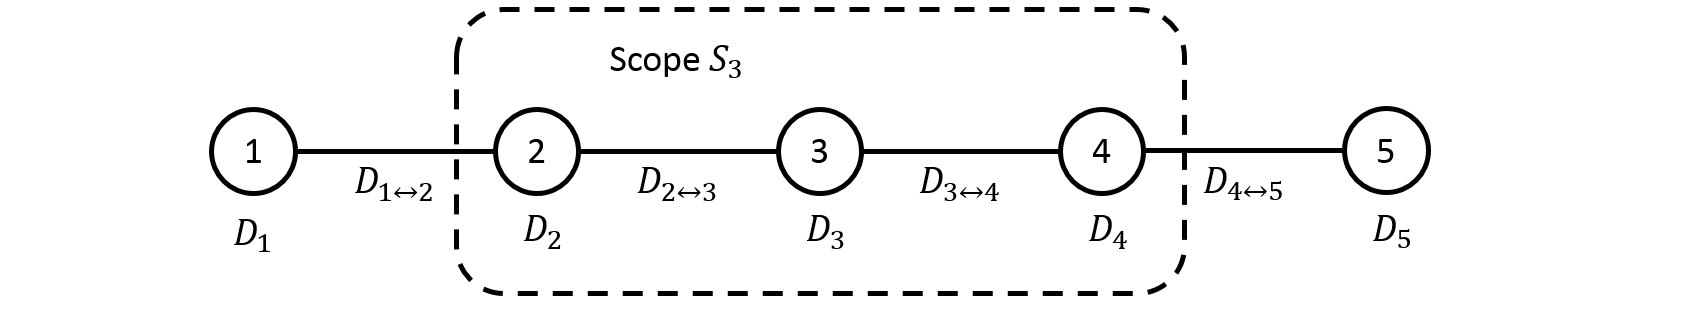
\includegraphics[width=\textwidth]{Scope.png}
    \caption{Scope $S_3$ of vertex 3}
    \label{fig:Scope}
  \end{center}
\end{figure}

In contrast to Pregel, in which the execution of vertex function is triggered by the messages and can access the data only in the messages, GraphLab separates the movement of the data and scheduling for execution. Therefore update function in GraphLab can access data of adjacent vertices even if the vertices are not scheduled. The update function in GraphLab gives user freedom to access the data of adjacent edges and vertices. By returning the scheduled vertices, GraphLab is able to express dynamic computation. 

Algorithm~\vref{alg:GraphLabExecutionModel}\cite{Low+al:uai10graphlab} shows the GraphLab execution model. The input to GraphLab are the data graph $G=(V,E,D)$ and an initial vertex set $T$ that are scheduled when the execution starts (line 1-2). While there exist vertices in the set $T$ (line 3), a vertex is removed from the set and the update function is executed, which updates the data within the scope and returns a set of scheduled vertices (line 4-5). The vertex set $T$ is updated, in which duplicated vertices are ignored (line 6). The output is the updated data graph. 

	\begin{Algorithmus}[H]
	\label{alg:GraphLabExecutionModel}
	\caption{GraphLab Execution Model}	
	\begin{algorithmic}[1]
	\State \textbf{Input}: Data Graph $G=(V,E,D)$
	\State \textbf{Input}: Initial vertex set $T$
	\While{$T \neq \emptyset$}
		\State $v \leftarrow RemoveNext(T)$
		\State $(S_v, T') \leftarrow f(v,S_v)$
		\State $T \leftarrow T \cup T'$
	\EndWhile
	\State \textbf{Output}: Modified Data Graph $G=(V,E,D')$
	\end{algorithmic}	
	\end{Algorithmus}

Due to asynchronous parallel execution in GraphLab, it must be avoided that update function of different vertices modify the data simultaneously. Otherwise, race condition may lead to non-deterministic behaviour. For example, non-deterministic happens, when both vertex 3 and vertex 4 in Figure~\ref{fig:Scope} try to write $D_{3 \leftrightarrow 4}$ in parallel. A serializable execution avoids executing overlapping computation at the same time. A serializable execution in GraphLab means that the scheduled parallel execution by Algorithm~\vref{alg:GraphLabExecutionModel} has a corresponding serial execution of update function that produces the same result. Therefore GraphLab introduces three consistency models as shown in Figure~\ref{fig:ConsistencyModel}. The full consistency model ensures each update function has exclusive read-write access to the vertex scope. The edge consistency ensures each update function has exclusive read-write access to the vertex and adjacent edges but read only access to adjacent vertices. The vertex consistency ensures each update function has exclusive read-write access to the vertex but read only access to adjacent edges. From full consistency to vertex consistency, the consistency degree is decreasing while the parallelism degree is increasing.

\begin{figure}[H]
  \begin{center}
    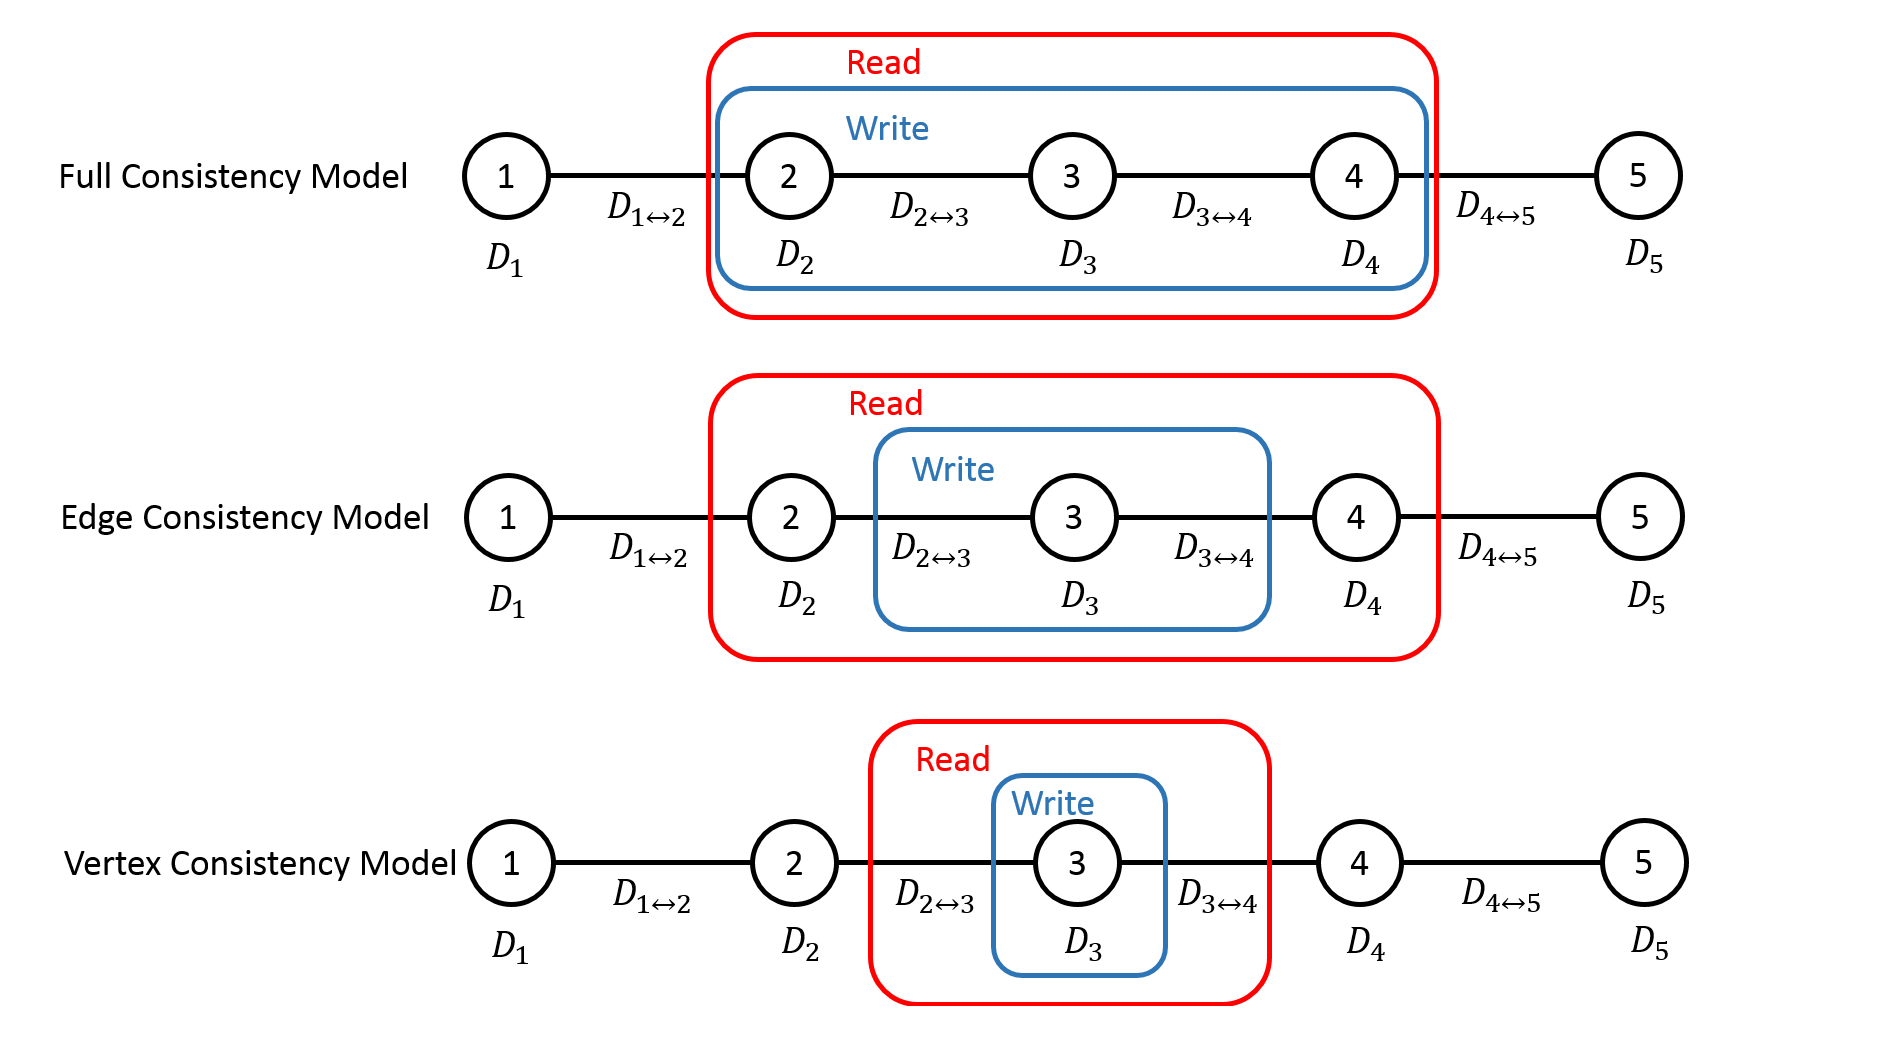
\includegraphics[width=\textwidth]{ConsistencyModel.png}
    \caption{Consistency models}
    \label{fig:ConsistencyModel}
  \end{center}
\end{figure}

The sync operation is similar to the aggregator in Pregel. In contrast to the aggregator, the sync operation has a finalization phase and runs continuously.

\subsection{Distributed GraphLab Architecture}

GraphLab uses a graph representation based on two-stage partitioning, which is efficient and balance to load graph on the cluster. Firstly the data graph is partitioned into many small pieces using domain specific knowledge or partitioning heuristic, which is much greater than the number of machines. Each piece is called an atom and stored separately on the distributed storage. The atom also stores the ghosts, which are the set of vertices and edges adjacent to the boundary. A meta-graph is created, in which vertices represent atoms. In second stage, GraphLab loads the meta-graph and distributes atoms over machines by a fast balanced partition. This technique allows the re-usage of graph partition.

GraphLab introduces two approaches to implementing the execution model. The \textit{Chromatic Engine} uses graph coloring that assigns each vertex with a color so that no adjacent vertices are assigned with the same color. The edge consistency is satisfied, when executing simultaneously all vertices of same color with a graph coloring. Other consistency model can also be satisfied by changing graph coloring. However the Chromatic Engine is not sufficient to flexibly schedule in many cases. The \textit{Locking Engine} extends the mutual exclusion in shared memory engine by associating readers-writer lock with each vertex. Different consistency models are implemented with different protocols.

GraphLab uses two approaches to creating snapshot for fault tolerance. To create a synchronous snapshot, execution is suspended, communication channels are flushed and all the data are saved to file-system. Asynchronous approach is based on the Chandy-Lamport snapshot, as the machines and channels in the Chandy-Lamport snapshot can be replaced by vertices and edges. The experiments also show that the asynchronous snapshot only slows down the execution, while the synchronous snapshot stops the execution.

\section{PowerGraph}

In \cite{gonzalez2012powergraph} the researchers point out that the natural graphs in the real world are characterized by highly skewed power-law degree distribution, which means most vertices have a few neighors while a few vertices have many neighbors. The probability of a vertex having degree $d$ under power-law distribution is:

\begin{equation}\label{eq:PowerLawDegree}
P(d) \propto d^{-\alpha}
\end{equation}

where $\alpha$ is a positive constant. In a highly skewed graph, the edges concentrate on a small fraction of vertices, which challenges the graph processing frameworks. The power-law degree distribution leads to partitioning difficulty and imbalance of communication, computation and storage. PowerGraph is proposed to address these problems by exploiting the characterization of the graph programs and the structure of the power-law graphs.

\subsection{The GAS Computation Model}

PowerGraph summarized the common features of the vertex function that are shared by both Pregel and GraphLab, and introduces the GAS model to characterize generality and differentiate the computation of vertices and edge. The GAS model represents three phase of a vertex function: \textbf{G}ather, \textbf{A}pply and \textbf{S}catter. 

PowerGraph offers an interface to implement algorithms in GAS model, which is shown in Figure~\ref{fig:GASVertexFunction} \cite{gonzalez2012powergraph}. The gather function is invoked on a set of adjacent edges of the vertex $u$ in parallel. The set of edges can be \emph{none}, \textit{in}, \textit{out} or \textit{all}, which is determined by \textit{gather\_nbrs}. The gather function collects the data and returns a temporary accumulator, which is then fed to the sum function to produce a final result $Accum$. The sum function inherits the commutative and associative gather concept from Pregel.

Based on the old vertex data $D_u$, the apply function uses the final result $Accum$ to update new vertex data $D^{new}_u$ which is saved to the graph by an atomic operation. The size of the accumulator $Accum$ and complexity of the apply function play a central role in determining the network and storage efficiency of the PowerGraph abstraction.
 
The scatter function is invoked on a set of adjacent edges determined by \textit{scatter\_nbrs}, which is same as in gather function. The scatter function may also update the data of the adjacent edges.

\begin{figure}
  \begin{center}
    
\includegraphics[width=\textwidth]{GASVertexFunction.png}
    \caption{GAS vertex function interface}
    \label{fig:GASVertexFunction}
  \end{center}
\end{figure}


%In the gather phase, the vertex gathers the information from adjacent edges and vertices. Then a commutative and associative sum operation $\oplus$ is performed on the gathered data:

%$$\forall v \in Nbr[u]: Accum \leftarrow \oplus gather(D_u,D_{(u,v)},D_v)$$

%The resulting data $Accum$ is used in apply phase to update the data of the current vertex. 

%$$D^{new}_u \leftarrow a(D_u,Accum)$$

%In the scatter phase, the new vertex data is used to update the data of adjacent edges.

%$$\forall v \in Nbr[u]: D_{(u,v)} \leftarrow scatter(D^{new}_u,D_{(u,v)},D_v)$$

A vertex becomes inactive after completion of the scatter phase but can be reactivated. A vertex can activate itself and the neighboring vertices. For example, in the PageRank a vertex gathers data from in-edges and uses the summed result to update its value and operates on out-edges in scatter phase. Further activation of vertices can be done in any GAS functions, but only the vertices that are visible in the specific function arguments. For example, a vertex can activate itself in apply function and neighbors in scatter function.

In Pregel and GraphLab abstraction the GAS model is expressed differently. Pregel uses message passing and combiner instead of the gather phase, and implements the apply phase and the scatter phase within vertex function. GraphLab allows user-defined vertex function to access entire information within the neighborhood.

\subsection{PowerGraph Architecture}

PowerGraph divides the vertex function into GAS model, so that it can express an algorithm in "think-like-a-vertex", and distribute the computation of a single vertex function over the cluster. %It inherits the commutative associative gather concept from Pregel and also borrows the data graph and shared-memory to keep user from specifying the data movement.
In addition, a vertex might be activated while a few of its neighbors are changed. However, the gather function is invoked on all neighbors. Therefore the gather function can be skipped for some algorithms by caching the accumulator and updating the accumulator with an optional $\Delta a$ returned by the scatter function. If the scatter function does not return $\Delta a$, then the cached accumulators of neighbors are cleared to force a complete gather phase on neighbors in next execution.

Algorithm~\vref{alg:PowerGraphExecutionModel} \cite{gonzalez2012powergraph} expresses the semantics how PowerGraph engine invokes GAS functions. The gather function is skipped if cached accumulator is empty. Otherwise the gather function is performed (line 2-6). The apply function uses the accumulator for update (line 7). In the scatter function, an optional returned $\Delta a$ is used to update the accumulator of each neighboring vertex, when both $\Delta a$ and neighboring accumulator are not empty. Otherwise, neighboring accumulator is set to empty (line 8-15).

	\begin{Algorithmus}[H]
	\label{alg:PowerGraphExecutionModel}
	\caption{PowerGraph Execution Model}	
	\begin{algorithmic}[1]
	\State \textbf{Input}: Center vertex $u$
	\If{cached accumulator $a_u$ is $empty$}
		\For{neighbor $v$ in $gather\_nbrs(u)$}
			\State $a_u \leftarrow sum(a_u,gather(D_u,D_{(u,v)},D_v))$
		\EndFor
	\EndIf
	\State $D_u \leftarrow apply(D_u,a_u)$
	\For{neighbor $v$ in $scatter\_nbrs(u)$}
		\State $(D_{(u,v)}, \Delta a) \leftarrow scatter(D_u,D_{(u,v)},D_v)$
		\If{$a_v$ and $\Delta a$ are not $empty$}
			\State $a_v \leftarrow sum(a_v, \Delta a)$
		\Else
			\State $a_v \leftarrow empty$
		\EndIf
	\EndFor	
	\end{algorithmic}	
	\end{Algorithmus}

The execution order of activated vertices depends on The PowerGraph engine. PowerGraph provides both synchronous engine and asynchronous engine. The synchronous engine executes each phase in order on all active vertices, which is synchronized with a barrier at the end of each phase. A superstep is defined as a complete series of GAS functions. The changes made in each phase are visible in the next phase. Vertices activated in each superstep are executed in the next superstep. Synchronous execution is similar to Pregel, which ensures a deterministic execution but limits the parallelism of the algorithms. The asynchronous engine can efficiently execute active vertices as long as resources are available, which accelerates the convergence of some algorithms. The changes on data of edges and vertices are immediately visible to neighbors in following computation. The asynchronous execution leads to non-deterministic, which is not suitable for some algorithms and is difficult for debugging. To retain the strong serializability, PowerGraph improves the locking protocol proposed in GraphLab, which is fair to high degree vertices. 

\subsection{Vertex Cut}

One way to place a graph on $p$ different machines is the balanced $p$-way edge-cut, which evenly assigns the vertices to different machine and minimizes the the number of edges spanning over machines. However, it does not work well with power-law graphs. Frameworks like Pregel and GraphLab usually use random hash to place vertices, which is easy and fast, but cuts most of the edges. Every spanning edge exacerbates the overhead of storage and communication, because both machines have to maintain a copy of the adjacent data and synchronize the data.

To reduce communication and balance workload, PowerGraph uses vertex cut to place the graph. Similarly a $p$-way vertex-cut evenly assigns edges to $p$ machines and aims at minimizing the number of vertices spanning over multiple machines. Figure~\ref{fig:EdgeCutVertexCut} demonstrates edge-cut and vertex-cut, which partitions the graph over two machines. The dashed vertices are the mirrors. The two-way edge-cut yields three vertices that are replicated on the two machines, while the two-way vertex-cut only yields one.

\begin{figure}
  \begin{center}
    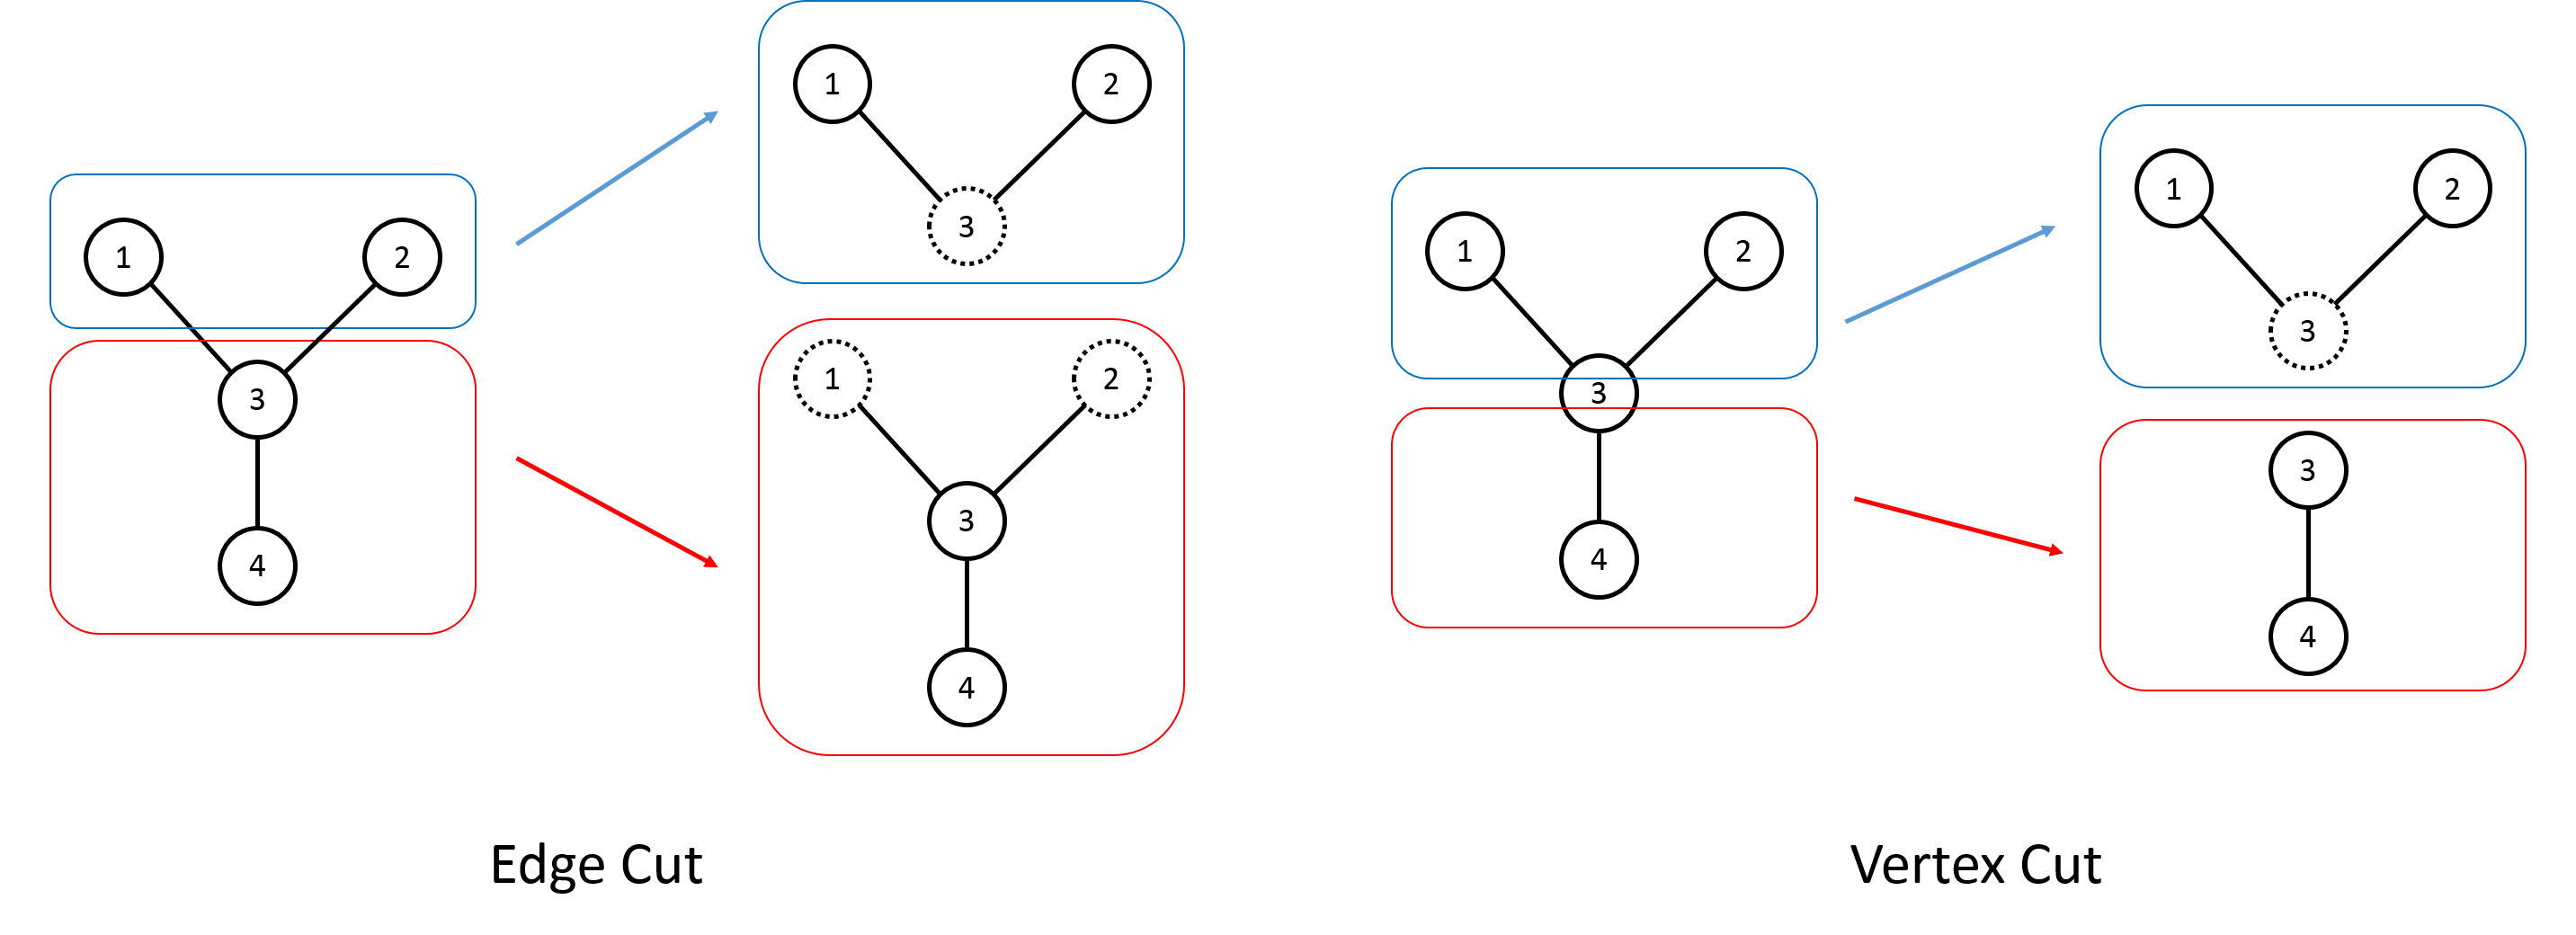
\includegraphics[width=\textwidth]{EdgeCutVertexCut.png}
    \caption{Demonstration of edge-cut and vertex-cut}
    \label{fig:EdgeCutVertexCut}
  \end{center}
\end{figure}

Therefore PowerGraph abstraction allows vertex as well as its vertex function to span over machines. Figure~\ref{fig:SplitVertexFunction} shows that a vertex function is split over two machines. The rectangles of gather, apply and scatter functions represent their execution region. By using vertex cut, massive edges are distributed over machines and each edge is stored on only one machine. Therefore modifications on edge data do not need communication. But modifications on vertex data must be committed to all the machine it spans. Therefore the number of machines that vertices span determines the storage and communication overhead.

\begin{figure}
  \begin{center}
    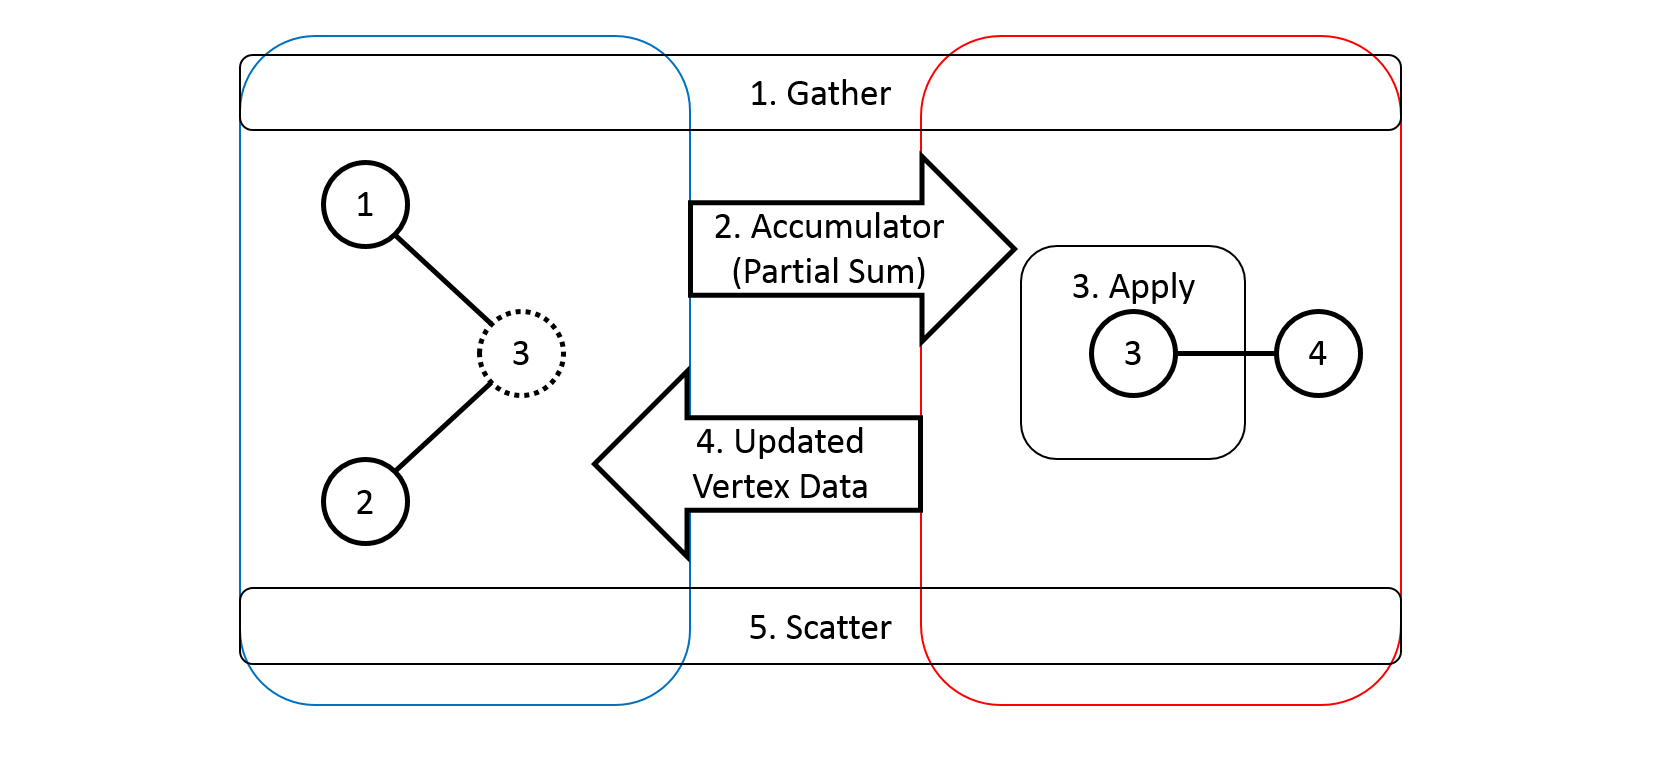
\includegraphics[width=\textwidth]{SplitVertexFunction.png}
    \caption{Vertex function that is split over two machines}
    \label{fig:SplitVertexFunction}
  \end{center}
\end{figure}


The term \textit{replicas} is used to denote the set of machines that a vertex spans. One of the replicas is randomly chosen as the \textit{master} that maintains the master version of the vertex data. The rest replicas are mirrors that only keeps a local copy of the vertex data. Modifications on the vertex data during apply phase are first made to the master and then copied to all mirrors.

Randomly assigning edges to machines is the simplest way to construct a vertex cut, which is completely data-parallel and can achieve a satisfactory result. Greedy-heuristic can be used to improve the result. Greedy-heuristic performs a sequential edge assignment by assigning the next edge on the machine which can minimize the conditional expected replication factor. Greedy-heuristic gives a result that is theoretically no worse than random edge assignment and often better in practice. However, greedy-heuristic needs coordination between machines. PowerGraph offers two implementations for the greedy-heuristic. In \textit{Oblivous}, each machine runs the greedy-heuristic independently and estimates replication factor locally. In \textit{Coordinated}, each machine communicates periodically on previous edge assignment to estimate replication factor.

The experiments show that greedy-heuristic results in a smaller replication factor than random placement, but with longer ingress time. The runtime scales linearly with replication factor. Therefore the greedy-heuristic improves overall runtime when PageRank has more than 20 iterations in the experiment.

\section{Other Graph Processing Frameworks}

There exist many other systems for graph processing, which are often based on a existing framework, and overcome some limitations or improve the performance. For example, GPS (for Graph Processing System)\cite{salihoglu2013gps} is similar to Pregel, while it features a dynamic repartitioning method during the execution. GPS is also optimized for skewed graphs by distributing adjacency lists of high-degree vertices across all machines.

In GraphX\cite{xin2013graphx} researchers argue that graph processing frameworks often have shortage in graph construction and transformation, so the following computations could be problematic. GraphX combines the best of both graph-parallel systems and data-parallel systems by using resilient distributed datasets to express graph computation efficiently. The Resilient Distributed Graph (RDG) was presented as a graph abstraction, which supports many operation on a graph. It uses a tabular data representation for the efficient vertex-cut partitioning. 

PowerLyra\cite{chen2015powerlyra} is motivated by the observation that most graph processing frameworks treat and process all vertices uniformly. This would incur imbalance of workload or communication for either high-degree vertices or low-degree vertices. Therefore PowerLyra introduces a computation engine that supports dynamic differentiated processing according to vertex degree. It also provides a balanced $p$-way hybrid-cut strategy with heuristics for efficient graph partitioning, which combines the best of edge-cut and vertex-cut. To improve the data access locality, PowerLyra proposes locality-conscious graph layout. As PowerLyra is implemented based PowerGraph, the algorithms designed on PowerGraph can be seamlessly executed on PowerLyra.


%The parallel BGL\cite{gregor2005parallel}

%GraphChi\cite{kyrola2012graphchi}

%Mizan\cite{khayyat2013mizan}
\chapter{Distributed Subgraph Isomorphism}
\label{chap:c3}

Subgraph isomorphism is the core problem of graph pattern matching, which has been widely applied in different areas such as social networks, computer vision, electronics and biology. However, no existing algorithm for subgraph isomorphism is designed for graph processing frameworks, on which algorithms are expressed in a vertex-centric way. 

In this chapter, we discuss the problem of graph pattern matching, and then we innovatively design an algorithm to solve the subgraph isomorphism problem in a distributed setting. We also analyse properties of the algorithm, so an optimized algorithm and a variant algorithm of approximate solution are proposed. At the end the implementation details are given.

\section{Background of Graph Pattern Matching}

As summarized in \cite{gallagher2006matching}, graph pattern matching is actually not a single problem, but a set of problems with respect to graph characteristics and matching requirements. The problems vary from the NP-complete subgraph isomorphism, which gives the matches having the strict link structure as the pattern, to looser constrains on the results, which only need to keep similar structure of the pattern. The problems also vary from structural matching to semantic matching, depending on whether the pattern and graph are typed/attributed or not. 

The basic problem of graph pattern matching is to find subgraphs that match the given pattern according to the given requirements. To formulate the problem, three elements are necessary.

\begin{enumerate}
\item A data graph $G=(V, E)$, where $V$ is the set of vertices, $E \subseteq V \times V$ is the set of edges. Vertices and edges can be typed. 
\item A pattern $P=(V_p, E_p)$, where $V_p$ is the set of vertices, $E_p \subseteq V_p \times V_p$ is the set of edges. Vertices and edges can be typed.
\item Matching criteria, which specifies the structural and/or semantic equality (e.g. subgraph isomorphism or graph simulation) between subgraph $G'$ and $P$. $G'=(V',E')$, where $E' \subseteq V' \times V'$, is a subgraph of $G$ if and only if $V'\subseteq V$ and $E'\subseteq E$.
\end{enumerate}

\subsection{Problem Variations}

As the three elements vary, the problems vary.

\textbf{Charateristics of graphs}

Graphs can be \textit{directed} or \textit{undirected}. A graph is directed when the edges distinguish the starting point and the ending point. In a directed graph, $(v_1,v_2)$ represents the edge from $v_1$ to $v_2$ and $(v_2,v_1)$ represents the edge from $v_2$ to $v_1$. In the undirected graph, $(v_1,v_2)$ and $(v_2,v_1)$ represent the same edge.

Graphs also differ in whether \textit{multiple edges} (with same direction, if in directed graph) between two vertices are allowed or not.

Some graphs specify different \textit{weights on edges}, i.e. the map, while other graphs ignore the weights or consider the homogeneous weights.

Graphs also differ in whether \textit{self-loops} are allowed or not. A self-loop is the edge from a vertex to itself.

A graph is \textit{connected} when there exists some path between any two vertices in the graph. Connected graphs are more general and algorithms on this kind of graphs can be easily applied to a set of unconnected graphs.

In some graphs, vertices or edges are \textit{typed} from a defined type set, e.g. a label function on vertices. This means the graphs are associated with semantics. Figure~\ref{fig:TypedDataGraphExample} shows an example of a typed graph. The graph represents a developing team in a software company. A vertex represents a team member with a type of his profession. The type set in this case includes Product Manager, Software Engineer, Quality Engineer, Database Engineer and Architecture Engineer. A directed edge from A to B denotes that A can assign tasks to B.

\begin{figure}[H]
  \begin{center}
    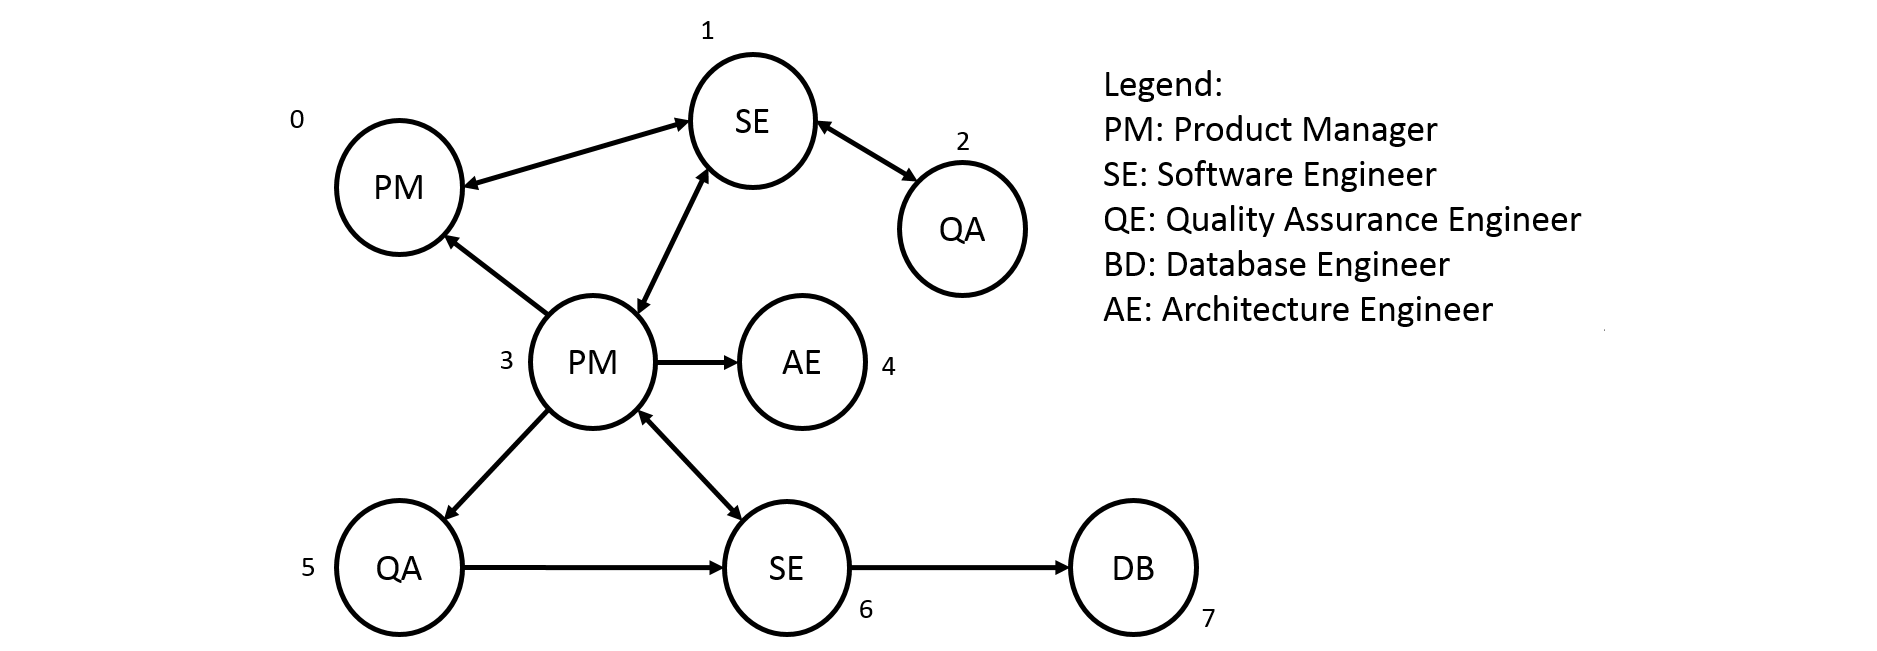
\includegraphics[width=\textwidth]{DataGraph.png}
    \caption{Typed graph with semantics}
    \label{fig:TypedDataGraphExample}
  \end{center}
\end{figure}

\textbf{Structual and semantic matching}

As graph can be either typed or untyped, some pattern matching algorithms are merely based on link structure of the graph and ignore the semantics of the graph. However, some pattern matching algorithms consider the semantics associated with typed vertices/edges of the graph as well as structure. 

\textbf{Exact and inexact matching}

Generally, pattern matching algorithms search subgraphs based on a specified pattern, and the results that match the pattern are in the same shape and have same semantics. This is the exact matching. However, in some situation, the pattern is partially specified, which is inexact matching (e.g. "find all triangle by ignoring the in/out edges"). Even the algorithms find the results that exactly match the pattern, but the results may be in different shape or have different semantics.

\textbf{Exact and approximate solutions}

Pattern matching algorithms vary on whether they guarantee the quality of the results they give. Algorithms for subgraph isomorphism guarantee the results to be optimal solution, if any, but they have been shown with an exponential worst-case complexity. Some algorithms give approximate results by loosing some constrains on the matching criteria, which are often with polynomial complexity. \cite{ma2011capturing} argues that graph isomorphism is sometimes to restrictive to catch sensible matches. To overcome this issue and to reduce the complexity, the several graph simulations are discussed, which actually fall into the category of approximate solutions.

\subsection{General Approach to Graph Pattern Matching}

The original subgraph isomorphism problem has been known as NP-complete\cite{gallagher2006matching}, so all known algorithms for subgraph isomorphism have the complexity of non-polynomial to the size of the input graph. Intuitively, a brute-force way of enumeration can be used to solve the problem. The brute-force enumeration procedure is a depth-first tree-search algorithm\cite{ullmann1976algorithm}.

To solve the problem in a reasonable time, many algorithms for subgraph isomorphism pre-process the data graph to filter the promising candidate for the actual matching processing. In \cite{giugno2002graphgrep, gallagher2006matching}, a basic frame is addressed to generalize this kind of approach. The frame consists of three steps: data analysis, candidate selection and matching. 

Pre-processing on the data graph can yield summary information, such as \textit{graph invariants}, which is helpful in data analysis and metadata construction. An invariant is a quantity to describe a graph. If two graphs are isomorphic, they must have the same invariants. Therefore, invariants can be easily used to compared between pattern and data graph to filter out unlikely matches. A canonical graph representation is used by some algorithms to generate invariants\cite{washio2003state}. In addition, some algorithms use statistical data as summary information\cite{getoor2011learning}.

The metadata of the graph directs candidate selection. If the pattern and a subgraph have different invariants or statistical data, it is unnecessary to perform further matching. If a graph are typed, there are lots of information available for candidate selection. For example, if the pattern contains a vertex of the type Product Manager, not every vertex but only the vertices of Product Manager in the graph should be considered as a potential match. The aim of the candidate selection is to provide a subset of data graph that contains all the potential matches for the matching phase.

In the matching phase, algorithms of structural or semantic matching approach are performed on the candidates to find the matches for the pattern.

\subsection{Distributed Graph Pattern Matching}

In recent years, frameworks, such as Pregel and PowerGraph, have been proposed for distributed graph processing. Many algorithms have been designed to fit this vertex-centric programming paradigm. However, as most algorithms for graph pattern matching are computation intensive, few can be performed on those distributed graph processing frameworks. In \cite{fard2013distributed}, a distributed vertex-centric approach is proposed for graph simulations. With the vertex-centric programming model, in contrast to usual graph programming models, an algorithm should be designed from the perspective of each vertex in a graph. This change from the point of view of vertices makes algorithm design more difficult for the problems like pattern matching that need a global overview of a graph.

To the best of our knowledge, no algorithm for subgraph isomorphism has been designed in vertex-centric way that can run on any of those frameworks yet.

\section{An Algorithm for Distributed Subgraph Isomorphism}

\subsection{Problem Formulation}

As the problem of graph pattern matching has many variations, a specific algorithm should describe what exact problem it can solve. An algorithm based on the GAS model of PowerGraph executed by a synchronous engine is proposed and referred to as DSI later to find isomorphic subgraphs in distributed computation. 

To formally define the subgraph isomorphism with semantics, assume that there is a data graph $G=(V, E, l)$ and a pattern $P=(V_p, E_p, l)$, where $l$ is label function on vertice, which assigns a label to a vertex. Subgraph isomorphism is to find subgraph $G_s=(V_s, E_s, l): V_s \subseteq V, E_s \subseteq E \cap (V_s \times V_s)$, so that there exists a bijective map $f_v : V_s \rightarrow V_p$ such that $(v_1, v_2) \in E_s \iff (f_v(v_1), f_v(v_2)) \in E_p$ and $l(v_1) = l(f(v_1))$ hold. We use $f_e$ to denote the bijective map between $E_s$ and $E_p$.

As PowerGraph can accept directed or undirected graph, no multiple edge, no self-loop, types on vertices or edges(or weights on edges) and connected or unconnected graph, DSI can solve the pattern matching problem, in which the data graph can be directed or undirected, can have types on vertices or edges, can be connected or unconnected, but must not have multiple edges or self-loops. DSI can accept the pattern having the same properties as data graph except that the pattern must be connected. This will not lose the generality, because all the connected parts of pattern can be performed on the same data graph, and the combination of the results will give the isomorphic subgraphs of the unconnected pattern.

DSI gives the exact solutions to exact matching, which can solve both structural and semantic matching problems.

\subsection{Algorithm Description}
\label{sec:dsi-des}

DSI thinks as vertex, which means each vertex knows only information of itself and its neighbors other than the whole data graph. The vertices receive, process and send messages, which are potential isomorphic subgraphs. The data types in DSI are data graph, pattern and message.

The pattern consists of vertices, and each vertex has:	
	\begin{itemize}
	\item A unique $ID_p$
	\item A label for typed graph
	\item Knowledge of the topological relation with neighboring vertices, i.e. what is direction of the edge(s) between it and a neighboring vertex
	\end{itemize}
The data graph consists of vertices, and each vertex has:
	\begin{itemize}
	\item A unique $ID_g$
	\item A label for typed graph
	\item Knowledge of the topological relation with neighboring vertices, i.e. what is direction of the edge(s) between it and a neighboring vertex
	\item Knowledge of the whole pattern
	\item Messages to process
	\end{itemize}	
The message has:
	\begin{itemize}
	\item Possible matching vertices pairs between the pattern and the data graph
	\item The source from where the message is sent
	\item A forwarding trace
	\end{itemize}

The idea behind the algorithm is that the messages representing potential matches go through the data graph and are processed by the vertices to find isomorphic subgraphs, as the vertices only have the local knowledge. The algorithm is explained in the fashion of message passing, which is easy to understand and to transform to the GAS model.

At the beginning, each vertex $v_g$ in the data graph generates a message with matching pair for its each possible matching vertex $v_p$ in the pattern, adds itself to the forwarding trace, and sends the messages to all neighbors.

On receiving messages, vertex $v_g$ uses the following operations on each message according to different situations. 
	\begin{itemize}
	\item \textbf{Forward:} If $v_g$ has matched a vertex in the pattern, it can not match any other pattern vertex. However, an updated message that has never been to $v_g$ should be passed to other possible vertices. In this case, if $v_g$ is not in the forwarding trace, then vertex function adds the vertex itself to the forwarding trace, and sends the message to all neighbors.
	\item \textbf{Update (Spawn):} If $v_g$ has not matched any vertex in the pattern and it can match to some neighbor of the vertex in the pattern, which the message source has matched, then for each possible matching vertex $v_p$, vertex function generates a new message based on the old one by adding the matching pair and replacing all IDs in the forwarding trace with the ID of the current vertex $v_g$. In this case, a message may spawn multiple new messages. If all the pattern vertices have been matched already after this operation in a new message, then an isomorphic subgraph has been found. Otherwise the messages are sent to all neighbors.
	\item \textbf{Drop:} In other situations, the message is dropped, because it is hopeless or redundant to find further matching vertex.
	\end{itemize}

The aim of using the forwarding trace is to avoid the out-of-date messages keeping alive infinitely. If a message is updated, it is fresh to every other vertex. The forwarding trace will be cleared and added with the current vertex ID. If a message is not updated, it can be forwarded by a vertex only once. So a message will die when it reaches the vertex that has seen the message. This mechanism guarantees that the algorithm terminates when there is no live message in the data graph.

In term of "match" between a vertex in the pattern and a vertex in the data graph, the criteria can be divided into structural criteria, which are defined in DSI, and semantic criteria, which can be defined differently for different scenarios. The structural criteria are that there is a bijective map from the vertices set of each subgraph to the vertices set of the pattern, and the edges set of a subgragh in the data graph must be the superset of the pattern. That is to say, if $v_g$ matches $v_p$, the adjacent edges of $v_g$ must be the superset of $v_p$'s adjacent edges. When a vertex $v_g$ checks whether it can match any $v_p$ on receiving a message, it is impossible to compare all the adjacent edges, because maybe not all neighboring vertices of $v_p$ in the pattern are matched. The alternative way to solve this problem is that $v_g$ ensures that the part of the adjacent edges between $v_g$ and previously matched vertices in the data graph are the superset of the part of the adjacent edges between $v_p$ and previously matched vertices in the pattern. As this condition is checked every time a new matching pair is added to the message, an isomorphic subgragh, if found, will keep the structural criteria.

DSI expressed in GAS form is shown as Algorithm~\vref{alg:GAS_DSI}. Messages are created or updated within the vertices. Instead of sending, a vertex gathers the messages from all neighbors in the gather phase (line 1-3). The sum operation aggregates all the messages (line 4-5). In the apply phase, the vertex firstly clears all messages of the last superstep (line 7). If the vertex function just starts, it generates a message with matching pair for each possible matching vertex in the pattern and adds itself to the forwarding trace (line 9). Otherwise it processes each gathered message. If the vertex exists in the matching pair and is not in the forwarding trace (line 12-13), \textbf{Forward} operation is used by adding vertex to the forwarding trace (line 14-15). Otherwise, the vertex uses \textbf{Update (Spawn)} operation. For each neighboring pattern vertex of the one that the message source (the last vertex in the forwarding trace) matches (line 18), the vertex compares matching criteria (line 19). If the vertex can match any, it spawns a new message based on the old one, and adds the matching pair and the forwarding trace (line 20-21). If all pattern vertices have been matched, an isomorphic subgraph is found, otherwise the new message is saved for next superstep (line 22-26). In the scatter phase, the vertex activates itself and all neighbors if there exist messages inside it (line 32-37). The reason to activate the vertex itself is to erase all messages even if no neighbor activates the vertex. Otherwise, the out-of-date messages might be gathered in the future iterations.

To execute the algorithm, the synchronous engine is necessary. Since a vertex will clear all its message before processing gathered messages, it should be guaranteed that all its neighbors gather its messages.


	\begin{Algorithmus}[H]
	\label{alg:GAS_DSI}
	\caption{Distributed Subgraph Isomorphism}	
	\begin{algorithmic}[1]
	
	\State //gather\_nbrs: ALL\_NBRS
	\State \textbf{gather}$(D_u, D_{(u,v)}, D_v)$: 
	\State \textbf{return} messages $D_v.ms$
	\newline
	\State \textbf{sum}$(ms_a, ms_b)$: 
	\State \textbf{return} $ms_a \cup ms_b$
	\newline
	\State \textbf{apply}$(D_u, gathered\_ms)$:
	\State $D_u.ms \leftarrow \emptyset$
	\If  {initialization}
		\State $\forall pv \in V_p, l(u)=l(pv)$: $D_u.ms \leftarrow D_u.ms \cup m$, where $m.pairs = \{(pv, u)\}$, $m.forwardingtrace = \{u\}$   
	\Else		
		\For	{message $m$ : $gathered\_ms$}
			\If  {$\forall (pu, gu) \in m.pairs, \exists gu: u = gu$}
				\If{$u \notin m.forwardingtrace$}
					\State $m.forwardingtrace \leftarrow m.forwardingtrace \cup \{u\}$ 
					\State $D_u.ms \leftarrow D_u.ms \cup m$
				\EndIf
			\Else
				\For {pattern vertex $pv$ : $f_v(m.forwardingtrace.last).neighbors$}
					\If {$\forall (pu, gu) \in m.pairs, \neg \exists pu: pu = pv$ \textbf{and} $\forall (pu, gu) \in m.pairs: f^{-1}_e(e(pv, pu)) \subseteq e(u,gu) $ \textbf{and} $l(u)=l(pv)$}
						\State $m'.pairs \leftarrow m.pairs \cup (pv,u)$
						\State $m'.forwardingtrace \leftarrow \{u\}$	
						\If {$|m'.pairs| = |V_p|$}
							\State $m'.pairs$ is a subgraph
						\Else
							\State $D_u.ms \leftarrow D_u.ms \cup pm'$
						\EndIf		
					\EndIf
				\EndFor		
			\EndIf
		\EndFor		
	\EndIf	
	\newline
	\State  //scatter\_nbrs: ALL\_NBRS
	\State \textbf{scatter}$(D_u, D_{(u,v)}, D_v)$:
	\If{$D_u.ms \neq \emptyset$}
		\State 	Activate($u$)
		\State 	Activate($v$)
	\EndIf

	\end{algorithmic}	
	\end{Algorithmus}

An example is given here to demonstrate how the algorithm works. Assuming that we are interested in finding a work group from the previous example of a team in a software company. So the pattern of the work group is shown in Figure~\ref{fig:BasicPattern}.

\begin{figure}[H]
  \begin{center}
    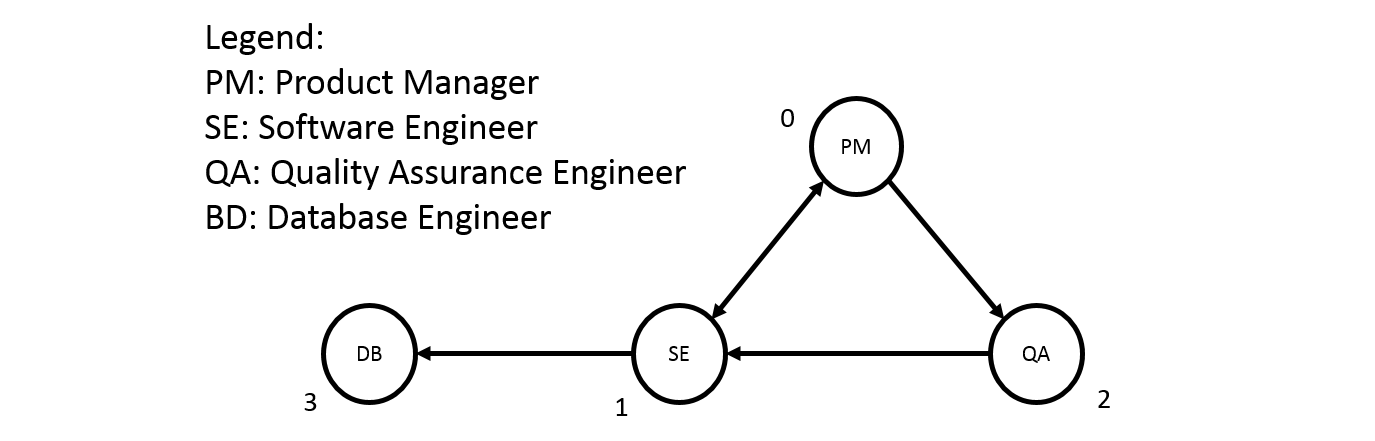
\includegraphics[width=\textwidth]{Pattern.png}
    \caption{Pattern with semantics}
    \label{fig:BasicPattern}
  \end{center}
\end{figure}

To simply and clearly illustrate the procedure of message passing and processing, only one message is created on the vertex 3 and passed through the data graph. The Figure~\ref{fig:MessagePassingDemo} shows the messages in each superstep. A message is denoted as \textbf{(matching IDs)[forwarding trace]}. The initial message (3,-1,-1,-1)[3] means that the data graph vertex 3 has matched to the pattern vertex 0, which is the position in the message. -1 in the message denotes that the pattern vertex has not been matched yet. And the data graph vertex 3 is in the forwarding trace. The message (3,-1,-1,-1)[3] is sent to all the neighboring vertices 0, 1, 4, 5 and 6.  The vertices 0 and 4 can not match any pattern vertex due to the semantic constrain, so they just simply drop the message. When vertex 5 receives the message (3,-1,-1,-1)[3], it checks the matching criteria, and it can match the pattern vertex 2, so it updates the message to (3,-1,5,-1)[5]. This updated message is also sent to all the neighboring vertices including vertex 3. In this case, vertex 3 only adds itself to the forwarding trace and the message becomes (3,-1,5,-1)[5,3]. When vertex 5 receives this message, it finds it is already in the message and the forwarding trace, so the message is dropped. Another example that violates the structural criteria is like this, when vertex 2 receives the message (3,1,-1,-1)[1], it tries to match the pattern vertex 2. However, it cannot keep the topological relation between pattern vertex 0 and 2, so it fails to match and drops the message. Some subgraphs are found in the vertices 5 and 7, which are actually duplicated.

\begin{figure}[H]
  \begin{center}
    
\includegraphics[width=0.64\textwidth]{MessagePassingTable.png}
    \caption{Message passing demonstration}
    \label{fig:MessagePassingDemo}
  \end{center}
\end{figure}

\section{Analysis of DSI}
After giving the description of the algorithm, we have to look at some critical properties of DSI. The algorithm must be correct and able to find all the isomorphic subgraphs, which are discussed in respect of correctness and completeness. We also have to make sure that the algorithm will terminate finally in a distributed environment. At last the complexity of DSI is analysed. After that we are able to know what is the bottleneck of DSI and try to make it more efficient.

\subsection{Correctness}

Here we prove that a subgraph found by the DSI satisfies the definition of the subgraph isomorphism.
 
Firstly, DSI guarantees the bijective map of vertices $f_v:V_s \leftrightarrow V_p$ between the subgraph and the pattern, as they have the same number of vertices and one data graph vertex can only match one pattern vertex. Secondly, the structural matching criteria guarantees topological relation between vertices $(v_1, v_2) \in E_s \iff (f_v(v_1), f_v(v_2)) \in E_p$. As the pattern is restricted to connected graph, the message passing mechanism guarantees that the local knowledge of vertices is enough to solve the problem. Finally, the semantic matching criteria guarantees matching pair has the same label $l(v_1) = l(f_v(v_1))$. 

\subsection{Termination and Deterministic}

As the forwarding trace strategy is used to avoid unchanged messages bounce in the graph infinitely, a message is either updated to an isomorphic subgraph finally or dropped when it cannot spread further. Here we show the maximum supersteps that DSI can have depending on the size of the given pattern, which size must be smaller than or equal to the size of data graph. The maximum number of vertices, to which a brand-new message can be passed (only for the first time) or forwarded without adding new matching pair, is the number of matching pairs in the message. It is the same for the maximum number that a brand-new message can walk among the vertices before a new pattern vertex becomes matched. Given a pattern having $k$ vertices, and a brand-new message with $i$ matching pairs, to find the $(i+1)th$ matching pair, the message at most go through $i$ vertices in the data graph. Therefore, the maximum of supersteps is:

\begin{equation}\label{eq:DSIComplexityMaxIteration}
\begin{split}
	S_{max} &= 1 + \sum_{i=1}^{k-1} i\\
			&= 1 + k*(k-1)/2\\
\end{split}
\end{equation}

The creation of the initial message takes one superstep. This is the upper bound of the superstep for a pattern of size $k$. However, the actual number might be lower, as a message can not walk through all the previously matched vertices because of the pattern topology.

The longest way to find a subgraph in the last example is 3 $\rightarrow$ 6 $\rightarrow$ 3 $\rightarrow$ 5 $\rightarrow$ 3 $\rightarrow$ 6 $\rightarrow$ 7, and corresponding message sequence is (3,-1,-1,-1)[3] $\rightarrow$ (3,6,-1,-1)[6] $\rightarrow$ (3,6,-1,-1)[6,3] $\rightarrow$ (3,6,5,-1)[5] $\rightarrow$ (3,6,5,-1)[5,3] $\rightarrow$ (3,6,5,-1)[5,3,6] $\rightarrow$ (3,6,5,7).

When creating initial messages, only semantic criteria has to be fulfilled, as it is not necessary to check the structural criteria for a single vertex. On receiving messages, both structural and semantic criteria are inspected between the current vertex and pattern vertices. When sending messages, the destinations are all neighbors. As creation, modification and transit of messages only depend on the given pattern and data graph, the outcome of DSI is deterministic.

\subsection{Completeness and Duplication}

DSI can find all the isomorphic subgraphs in the data graph. Messages are created and updated with the data graph.	Each message goes through the data graph until either a subgraph is found or the message is dropped. If there is any isomorphic subgraph, some messages will definitely go through it. As the pattern is restricted to a connected graph, we don't need to worry about the combination of the subgraphs.

However, it can be observed that the isomorphic subgraphs found in the ending vertices are highly duplicated. The reason is that some messages walk through different routes but end with the same subgraph, which is subject to only having the local knowledge in a distributed environment.

\subsection{Complexity}

Given a data graph of size $n$ and a pattern of size $k$, in the initial (first) superstep, each vertex tries to match every possible pattern vertex, so at most $k$ messages can be created. In the first superstep, the upper bound of complexity is:

\begin{equation}\label{eq:DSIComplexityInitial}
	T_1(n,k) = n*k
\end{equation}

In the $ith$ superstep, there are at most $n$ active vertices, each of which has at most $n-1$ neighbors. In each vertex, there can be at most $k*(n-1)^{i-1}$ messages to be processed by its neighbors. To process a message, all the previous matched vertices have to be checked, which are at most $(k-1)$. Therefore, in the $ith$ superstep, the upper bound of complexity is:

\begin{equation}\label{eq:DSIComplexityIth}
	T_i(n,k) = n*(n-1)*k*(n-1)^{i-1}*(k-1)
\end{equation}

In equation~\ref{eq:DSIComplexityMaxIteration} we have shown the maximum supersteps that DSI can run. Therefore the upper bound of total complexity is:

\begin{equation} \label{eq:DSIComplexityTotal}
	\begin{split}
		T(n,k) &= n*k + \sum_{i=2}^{1+k*(k-1)/2} n*(n-1)*k*(n-1)^{i-1}*(k-1)\\
		&= n*k*(1+(k-1)*\sum_{i=2}^{1+k*(k-1)/2} (n-1)^{i})\\
		&= n*k*(1+(k-1)*(\frac{(n-1)^2*((n-1)^{k*(k-1)/2}-1)}{n-2}))\\
	\end{split}
\end{equation}

As known already, subgraph isomorphism is a NP-complete problem, which depends both on the size of the input data graph and the pattern. Because we solve the problem in the distributed environment, it is inevitable to add more complexity.

\section{Optimizations}

One reason for that DSI has high complexity is that messages boost so fast while passing. Eliminating impossible or redundant messages without violating the essential properties of DSI will make DSI more efficient. The term \textit{optimized DSI} is used from now on to refer the algorithm with following optimizations.

\subsection{Constrains on Vertex Degree}
The graph invariants, the in and out degree of vertex, can be used to reduce the impossible messages. If the in or out degree of a data graph vertex is less than a pattern vertex, it is impossible to match those two vertices. So comparing the vertex degree is very helpful, when a vertex tries to match a pattern vertex. In this case, we reduce the messages that are not only created in the initialization but also on processing. Although it can not change the theoretical upper bound of complexity, it practically improves the efficiency of the algorithm.

Algorithm~\vref{alg:GAS_DSI_Degree} with constrains on vertex degree is based on the GAS representation of the original DSI. Here we only highlight the optimized part. The vertex function compares the in and out degree at the initialization (line 7) and when trying to add new matching pair (line 10).

	\begin{Algorithmus}[H]
	\label{alg:GAS_DSI_Degree}
	\caption{Optimized DSI on Vertex Degree}	
	\begin{algorithmic}[1]
	\State \textbf{gather}$(D_u, D_{(u,v)}, D_v)$: 
	\State ...
	\newline
	\State \textbf{sum}$(ms_a, ms_b)$: 
	\State ...
	\newline
	\State \textbf{apply}$(D_u, gathered\_ms)$:
	\If  {initialization}
		\State $\forall pv \in V_p, l(u)=l(pv), in-degree(u) \geq in-degree(pu), out-degree(u) \geq out-degree(pu)$: $D_u.ms \leftarrow D_u.ms \cup m$, where $m.pairs = \{(pv, u)\}$, $m.forwardingtrace = \{u\}$   
	\Else	
		\State ...
			\If {$\forall (pu, gu) \in m.pairs, \neg \exists pu: pu = pv$ \textbf{and} $\forall (pu, gu) \in m.pairs: f^{-1}_e(e(pv, pu)) \subseteq e(u,gu)$ \textbf{and} $in-degree(u) \geq in-degree(pu), out-degree(u) \geq out-degree(pu)$ \textbf{and} $l(u)=l(pv)$}
				\State ...
			\EndIf
		\State ...
	\EndIf
	\newline
	\State \textbf{scatter}$(D_u, D_{(u,v)}, D_v)$:
	\State ...

	\end{algorithmic}	
	\end{Algorithmus}

\subsection{Optimization of Initialization}

If we use the naive method to solve the subgraph isomorphism with a brute-force way of enumeration, we can start enumerating from any vertex, which will not effect the final results. It also makes sense that all vertices just try to match only one specific pattern vertex. This specific initial pattern vertex must be identical, which ensures that at least one message is created within each isomorphic subgraph if any. In the previous example, all the vertices may try to match the pattern vertex 3, so only one message is created in vertex 7 and the subgraph (3,6,5,7) will finally be found. It might not work, for instance, when all the vertices except 7 try to match the pattern vertex 3, but vertex 7 tries to match the pattern vertex 0.

As all the isomorphic subgraphs must contain the matching vertex of the specific initial one, the completeness of the algorithm will not be affected and the duplication of the results will be decreased. In this case, we reduce the messages that are created in the initialization and reduce the upper bound of complexity to:

\begin{equation}\label{eq:DSIComplexityOptimized}
	T(n,k) = n*(1+(k-1)*(\frac{(n-1)^2*((n-1)^{k*(k-1)/2}-1)}{n-2}))
\end{equation}


Choosing different initial pattern vertex may lead to different performance, including duplication degree, the number of messages, communication and etc.. 

Algorithm~\vref{alg:GAS_DSI_Initial} with the optimization of initialization is based on the GAS representation of the original DSI. Here we only highlight the optimized part. The vertex function only tries to match an identical vertex at initialization (line 8).

	\begin{Algorithmus}[H]
	\label{alg:GAS_DSI_Initial}
	\caption{Optimized DSI on Initialization}	
	\begin{algorithmic}[1]
	\State \textbf{gather}$(D_u, D_{(u,v)}, D_v)$: 
	\State ...
	\newline
	\State \textbf{sum}$(ms_a, ms_b)$:
	\State ...
	\newline
	\State \textbf{apply}$(D_u, gathered\_ms)$:
	\State $D_u.ms \leftarrow \emptyset$
	\If  {initialization}
		\State Select an identical $pv \in V_p, l(u)=l(pv)$: $D_u.ms \leftarrow D_u.ms \cup m$, where $m.pairs = \{(pv, u)\}$, $m.forwardingtrace = \{u\}$
	\State ...
	\EndIf
	\newline
	\State \textbf{scatter}$(D_u, D_{(u,v)}, D_v)$:
	\State ...
	\end{algorithmic}	
	\end{Algorithmus}
	
The GAS representation of the optimized DSI is easily deduced by merging the conditions of optimizations. 

\section{Balance Between Algorithm Complexity and Completeness}

The subgraph isomorphism problem is well known as a NP-complete problem and  algorithms for finding isomorphic subgraphs are exponential in
the size of the input graphs. Having exponential complexity, algorithms can not give results within an acceptable time and also might exhaust computing resource when processing large graphs. Sometimes an algorithm that gives a compromising solution with polynomial time complexity is desired, so that the execution time and the resource consumption are guaranteed. Alternatives are approximate solutions with polynomial time complexity, which are not guaranteed to find isomorphic subgraphs.

\subsection{Proportional Distributed Subgraph Isomorphism}

As we observe that in the equation~\ref{eq:DSIComplexityIth}, the upper bound of messages grows theoretically by multiplying $N-1$ after each superstep. We can turn the original solution into an approximate solution with polynomial time complexity, if we can make the factor to a constance. An alternative is proposed here called Proportional Distributed Subgraph Isomorphism (PDSI), which makes compromise between complexity and completeness. Based on the optimized DSI, PDSI differs in that the vertex function only randomly gathers a subset of messages in each neighboring vertex. Therefore, the complexity of the algorithm is significantly reduced. 

PDSI in GAS form is shown in Algorithm~\vref{alg:GAS_PDSI}. We only highlight the part that is modified. The vertex function only randomly gathers a subset of messages in each neighboring vertex (line 2).

	\begin{Algorithmus}[H]
	\label{alg:GAS_PDSI}
	\caption{Proportional Distributed Subgraph Isomorphism}	
	\begin{algorithmic}[1]
	\State \textbf{gather}$(D_u, D_{(u,v)}, D_v)$: 
	\State \textbf{return} Partial message set $ms'$, where $ms' \subseteq D_v.ms$ and $|ms'| = |D_v.ms|*p$, $p \in [0,1]$ is the proportion.
	\newline
	\State \textbf{sum}$(ms_a, ms_b)$:
	\State ...
	\newline
	\State \textbf{apply}$(D_u, gathered\_ms)$:
	\State ...
	\newline
	\State \textbf{scatter}$(D_u, D_{(u,v)}, D_v)$:
	\State ...

	\end{algorithmic}	
	\end{Algorithmus}

%In practice, we can not know \textbf{TODO}

\subsection{Properties of PDSI}

The subgraphs found by PDSI, if any, are still isomorphic to the given pattern, since we don't change the matching criteria. The theoretical upper bound of supersteps is not changed either. But PDSI is not guaranteed to find isomorphic subgraphs, because the necessary routes might not be traversed, which has another effect that the redundant messages are reduced as well.

The parameter $p$ is introduced to denote the proportion of the messages to be gathered in a neighboring vertex. In the $ith$ superstep, there are in total at most $n*(p*(n-1))^i*(k-1)$ messages to be processed. Therefore the upper bound of  the complexity is:

\begin{equation}\label{eq:PDSIComplexity}
	\begin{split}
		T(n,k,p) &= n*(1+(k-1)*\sum_{i=2}^{1+k*(k-1)/2} (p*(n-1))^{i})\\
		&= n*(1+(k-1)*(\frac{(p*(n-1))^2*((p*(n-1))^{k*(k-1)/2}-1)}{n-2}))\\
	\end{split}
\end{equation}

\section{Implementation}

In this section, we give more details about how the proposed algorithms are implemented in PowerGraph. The only essential methods and attributes for algorithms are listed. Functions such as \textit{save()} and \textit{load()}, which are necessary for serialization in PowerGraph are not listed.

The original DSI, optimized DSI and PDSI share the data types in Pattern Vertex, Data Graph Vertex and Message, while they differ in GAS functions.

\subsection{Pattern Vertex}

A pattern vertex should have properties which are mentioned in Section \ref{sec:dsi-des}. The abstract of class PatternVertex is shown in Listing~\ref{lst:PatternVertex}. The attributes are the information of vertex itself and four vectors of neighbors' IDs in different categories. Four methods are used to determine the topological relations between pattern vertices, and then to compare with data graph vertices.

\begin{Listing}[H]
\begin{lstlisting}
class PatternVertex
{
//methods
public:
	bool IsTarget(int id) const;
	bool IsSource(int id) const;
	bool IsNeighbor(int id) const;
	bool IsBi(int id) const;
//attributes
public:
	int id;
	string label;
	unsigned int in_degree;
	unsigned int out_degree;	
	vector<int>	targets;
	vector<int> sources;
	vector<int> neighbors;
	vector<int>	bidirected_neighbors;
};
\end{lstlisting}
\caption{PatternVertex}
\label{lst:PatternVertex}
\end{Listing}

\subsection{Pattern}

The pattern is loaded from a file. User should specify the format of the file and how to interpret. It is also necessary to specify whether the pattern is attributed or not.

\begin{Listing}[H]
\begin{lstlisting}
class Pattern
{
//methods
public:
	bool CreatePattern(string file, bool attributed);
//attributes
public:
	vector<PatternVertex> m_pattern;
};
\end{lstlisting}
\caption{Pattern}
\label{lst:Pattern}
\end{Listing}

\subsection{Message}

A message should store the matching pairs. In practice, we just use a vector to store the data graph vertices ids in a matching order. For example, the vertex, which ID is stored in the first place, matches the first pattern vertex. If a pattern vertex has not been matched yet, -1 is used as a placeholder. A message also has a vector to store the forwarding trace, in which the last one is the message source.

\begin{Listing}[H]
\begin{lstlisting}
typedef std::vector<graphlab::vertex_id_type> IDVector;

class Message
{
//attributes
public:
	IDVector matched_id;
	IDVector forwarding_trace;
};
\end{lstlisting}
\caption{Message}
\label{lst:Message}
\end{Listing}

\subsection{Data Graph Vertex}

A vertex in the data graph is similar to a pattern vertex. In addition, it has more data. The step indicator indicates which stage the vertex function is in. Because in PowerGraph vertex can only directly access the data in adjacent edges, so we use an additional superstep \textit{GetReady} to gather the IDs of the neighboring vertices. \textit{FirstStep} indicates the initialization stage and \textit{SecondStep} is the stage of message processing. Each vertex also contains a local copy of the pattern. The \textit{messages\_in\_vertex} is used to store the messages and the \textit{matched\_subgraphs} stores the isomorphic subgraphs. 

\begin{Listing}[H]
\begin{lstlisting}
enum StepIndicator {GetReady = 0, FirstStep, SecondStep};

class DataGraphVertex
{
//methods
public:	
	bool IsTarget(graphlab::vertex_id_type id) const;
	bool IsSource(graphlab::vertex_id_type id) const;
	bool IsNeighbor(graphlab::vertex_id_type id) const;
	bool IsBi(graphlab::vertex_id_type id) const;
//attributes
public:
	string label;
	Pattern local_pattern;
	StepIndicator si;
	MessagesInVertex messages_in_vertex;
	vector<IDVector> matched_subgraphs;	
	IDVector	targets;
	IDVector 	sources;
	IDVector 	neighbors;
	IDVector	bidirected_neighbors;
};
\end{lstlisting}
\caption{DataGraphVertex}
\label{lst:DataGraphVertex}
\end{Listing}

%\subsection{GAS Functions}
\chapter{Geospatial Simulation Using Agent-Based Cellular Automata}
\label{chap:c4}

Understanding complex dynamics of our society and the environment we live in can give direction to solve social issues and contribute to global sustainability. Therefore, we study the problem of geospatial simulation in this chapter. Firstly we describe the agent-based cellular automata model, which is used for our simulation. Then we show that graph processing frameworks are adequate for large scale geospatial simulation, and propose a simulation algorithm. At the end the implementation details are given.

\section{Background of Simulation Models}

The geo-informatics with spatial and temporal data have assisted the investigation and modelling the environmental systems. Simulations are performed depending on different scenarios and objectives. Mobile entities such as vehicles and people move along their trajectories over a given space and time span. Simulations such as traffic simulation and pedestrian simulation are appropriate for these scenarios. 

Mathematical models in macroscopic simulation of this kind of behaviour have been studied for decades. However this approach is inappropriate to capture details as compared to the models that simulate in microscope, such as cellular automata or agent-based model. A profound impact on the whole system may be caused by a perturbation of an agent's action that leads to cascading effects\cite{suzumura2014towards}.

Cellular Automaton (CA) is a discrete spatio-temporal model, which is widely used in simulation of various real-world systems, such as social simulation. Cellular Automata consist of a regular grid of cells, each of which is in one of finite states. Each cell has a set of cells as \textit{neighborhood}, which is spatial relative to the cell. Each cell is assigned with an initial state. The next state of a cell is determined by some fixed rules depending on the current state of itself as well as its neighborhood. Typically the rule for updating the state of cells is same for every cell and does not change over time, and is applied to all cells simultaneously.

A typical example is two-dimensional cellular automata as a sheet of graph paper, in which each square represents a cell with its state and the rules to follow. The neighborhood is usually adjacent cells. The most common neighborhoods shown in Figure~\ref{fig:Neighborhood} are the von Neumann neighborhood, which is the four orthogonally adjacent cells, and Moore neighborhood, which is the eight surrounding cells. For example, the state of a cell is either white or black and the next state is determined by the dominant color of the neighborhood.

\begin{figure}
  \begin{center}
    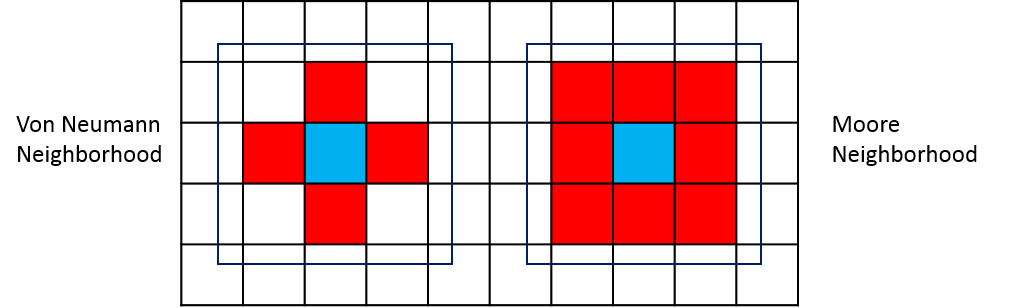
\includegraphics[width=\textwidth]{Neighborhood.png}
    \caption{Von Neumann neighborhood and Moore neighborhood}
    \label{fig:Neighborhood}
  \end{center}
\end{figure} 

Agent-based model (ABM) is a computational model for simulating the actions and interactions of multiple agents. An agent is an autonomous entity with self-contained program that is capable to perceive, decide and react on the environment. Agent-based model gives explanatory view on the collective behaviour and the effects of agents on the system as a whole. Agent-based model is a microscale model, which simulates the simultaneous actions and interactions of multiple agents to re-build or predict the occurrence of complicated phenomena. The process is reflection from micro level of the system to macro level, as the simple behavioural rules of agents lead to complicated behaviour of the system. ABM is able to represent and simulate more complicated and dynamical systems than CA.

Agent-Based Cellular Automata (ABCA)\cite{sudhira2005framework} is an integration of CA and ABM, which is capable to represent both spatio-temporal and agent dynamics. CA offsets the limitation of ABM to express the topology or the spatial relationships in the geographic perspective, and ABM brings the dynamics. In ABCA, agents are used to simulate the geographic objects in two-dimensional Euclidean space, so the definitions of the objects are points, lines and polygons. Agents move inside cells that define the transition rule. A cell reflects its local situation, and the collective effects of the cells contribute to observation as a whole.

ABCA is adequate for mobile-agent-based simulation, as interactions of agents are local in a cell. The parallel distributed computing system is ideal to execute this kind of simulation with large-scale datasets. In \cite{suzumura2012highly}, highly scalable X10-based agent simulation  platform XAXIS was used to simulate millions of agents in traffic flow simulation.

When geospatial simulation runs in Agent-Based Cellular Automata, a virtual space is composed of an array of cells, in which autonomous agents move around. When an agent goes beyond the border of its current cell, it migrates to the adjacent cell. The state of the cell changes with respect of to the agents inside it. 

\section{Simulation in Graph Processing Framework}

With the nature of the model, Agent-Based Cellular Automata is able to run on distributed systems like graph processing frameworks by partitioning the virtual area on distributed machines. Each machine has a set of cells, in which agents move round.

The simulation is pretty straightforward. The agents are initialized and the states of cells are based on their residing agents. Then the agents in the current cell update their locations. If the new location of a agent is beyond the area of the cell, it will migrate to the neighbor. Otherwise, the agent still resides in the current cell.

An agent becomes inactive and is removed when it can not update it location any more, and a cell becomes inactive when there is no active agent inside it. Therefore the simulation terminates when no agent exists and hence all cells are inactive.

The geospatial simulation using ABCA in GAS form is shown in Algorithm~\vref{alg:GAS_ABCA}. In the gather phase, the migrating agents from CA neighborhood of the current cell are gathered (line 1-3). The sum operation aggregates all migrating agents (line 4-5). In the apply phase, the vertex function merges its residing agents and the gathered agents, and clears all migrating queues (line 7-8). Then the vertex function updates the locations of its residing agents. If an agent moves beyond the current vertex, then the vertex function removes the agent and adds it to the corresponding queue (line 10-16). In the scatter phase, the vertex function activates itself, if it still has agents inside, and activates a neighbor, if the migrating queue of that neighbor is not empty (line 17-24).

The synchronization issue of ABCA is easily solved by using the synchronous engine. The algorithm can simulate with an arbitrary time interval specified by the user, and the synchronous engine guarantees the correctness of the spatio-temporal state. The collective effect of agents moving without conflict gives a view of the current situation in the macroscale.

	\begin{Algorithmus}[H]
	\label{alg:GAS_ABCA}
	\caption{Agent-Based Cellular Automata}	
	\begin{algorithmic}[1]
	\State //gather\_nbrs: IN\_NBRS
	\State \textbf{gather}$(D_u, D_{(u,v)}, D_v)$: 
	\State \textbf{return} agents $D_v.queue_u$
	\newline
	\State \textbf{sum}$(queue_a, queue_b)$: 
	\State \textbf{return} $queue_a \cup queue_b$
	\newline
	\State \textbf{apply}$(D_u, gathered\_agents)$:
	\State $D_u.queue_u \leftarrow D_u.queue_u \cup gathered\_agents$
	\State $\forall v \in u.neighbors, D_u.queue_v \leftarrow \emptyset $
	\State u.updateAgentsLocation()
	\For{agent $a$: $gathered\_agents$}
		\If{$u \neq a.destination$}
			\State $v \leftarrow a.destination$
			\State $D_u.queue_u \setminus \{a\}$
			\State $D_u.queue_v \cup \{a\}$
		\EndIf
	\EndFor
	\newline	
	\State //scatter\_nbrs: OUT\_NBRS
	\State \textbf{scatter}$(D_u, D_{(u,v)}, D_v)$: 
	\If{$D_u.queue_v \neq \emptyset$}
		\State 	Activate($v$)
	\EndIf
	\If{$D_u.queue_u \neq \emptyset$}
		\State 	Activate($u$)
	\EndIf
	\end{algorithmic}
	\end{Algorithmus}

\section{Implementation}

\subsection{Agent}

In our implementation, agents are simplified to points, which can be different, e.g. a shaped objects in other scenarios. An agent has its current coordinates and status as attributes, and agent updates its next coordinates according to the rule expressed in \textit{UpdateLocation()} method.

\begin{Listing}[H]
\begin{lstlisting}
enum AgentStatus { Unstarted = 0, Moving, Stopped };

class Agent
{
//methods
public:
	bool UpdateLocation();
//attributes		
public:
	double x;
	double y;
	AgentStatus agent_status;
};
\end{lstlisting}
\caption{Agent}
\label{lst:Agent}
\end{Listing}

\subsection{Cellular Automaton}

A cellular automaton should know its geographical space and the IDs of the neighbors, and it uses a vector of agent to hold inside agents and a map to hold the agents that migrate to the neighbors. Moore neighborhood is chosen to express the topology in our implementation. 

\begin{Listing}[H]
\begin{lstlisting}
class CellularAutomata
{
//attributes	
public:
	double space_top;
	double space_bottom;
	double space_left;
	double space_right;	
	vector<graphlab::vertex_id_type> neighbor_id;	
	vector<Agent> agents;
	map<graphlab::vertex_id_type, vector<Agent>> agents_to_target;
};
\end{lstlisting}
\caption{CellularAutomaton}
\label{lst:CellularAutomaton}
\end{Listing}

%\subsection{GAS Functions}
\chapter{Evaluation}
\label{chap:c5}

In this chapter evaluation of proposed algorithms on two different graph processing frameworks is elaborated. Firstly we evaluate the properties and performance of the algorithms for subgraph isomorphism on PowerGraph. Secondly we show the heterogeneity of the communication costs for vertex synchronization in the problems of both subgraph isomorphism and geospatial simulation. At the end we use these algorithms to show GrapH outperforms PowerGraph with respect to communication.

The experiments were conducted on a cluster of 11 machines, each of which has 3.0GHz Intel Xeon CPU E5472 with 8 cores, and 32GB RAM. The machines are connected with 1 Gbps Ethernet.

\section{Evaluation of DSI and its variants on PowerGraph}

To evaluate the algorithms for subgraph isomorphism, we use the real-life datasets\footnote{http://snap.stanford.edu/data/index.html}: (a) Wiki-Vote records Wikipedia who-votes-on-whom network, which is a directed graph with 7,115 nodes and 103,689 directed edges. (b) ego-Twitter records social circles from Twitter, which is a directed graph with 81,306 nodes and 2,420,744 directed edges. In the experiments of this section, vertices are randomly assigned with a label from a label set of 5 distinct elements.

\subsection{Impact of Pattern Size}

The experiments are started with a random pattern and proceeded by adding vertices one by one and adding edges between the vertices. The size of the pattern varies from 2 vertices to 5 vertices. Our cluster is not able to execute when the pattern size reaches 6, as all the memories are exhausted. The data graph is Wiki-Vote, and the number of machines is 11. For optimized DSI and PDSI, the initial vertex is randomly chosen. For PDSI, the parameter proportion is 0.3. 

We evaluate the runtime and message amount of these three algorithms with different pattern sizes. Figure~\ref{fig:runtime-P} shows that the runtime of DSI and optimized DSI increases drastically as the pattern size grows, as the computational complexity is exponential to the pattern size. With two optimization strategies, the optimized DSI only takes about one third runtime as DSI needs. The runtime of PDSI does not increase so much as the boost of messages is limited by the proportion.

\begin{figure}[H]
  \begin{center}
    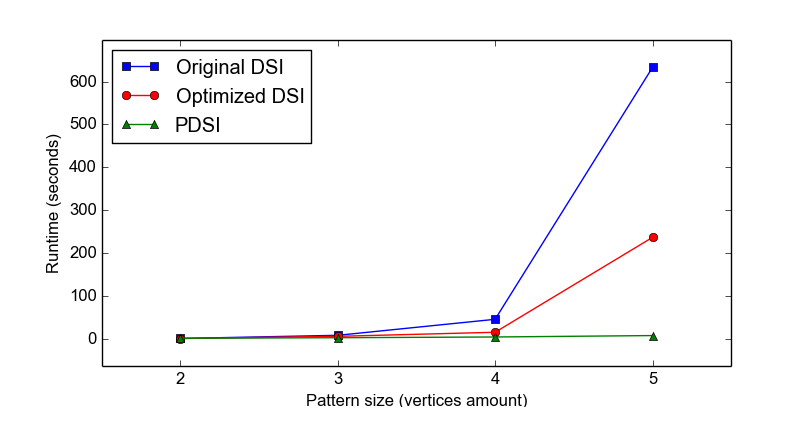
\includegraphics[width=\textwidth]{runtime-P.png}
    \caption{Runtime of DSI, optimized DSI and PDSI with patterns of different sizes}
    \label{fig:runtime-P}
  \end{center}
\end{figure}

Figure~\ref{fig:messages-P} shows that total message amount generated during the execution. The message amount is exponential to the pattern size. The runtime increases with same rate as the message amount grows, as the runtime mainly depends on how many messages to be processed.

\begin{figure}[H]
  \begin{center}
    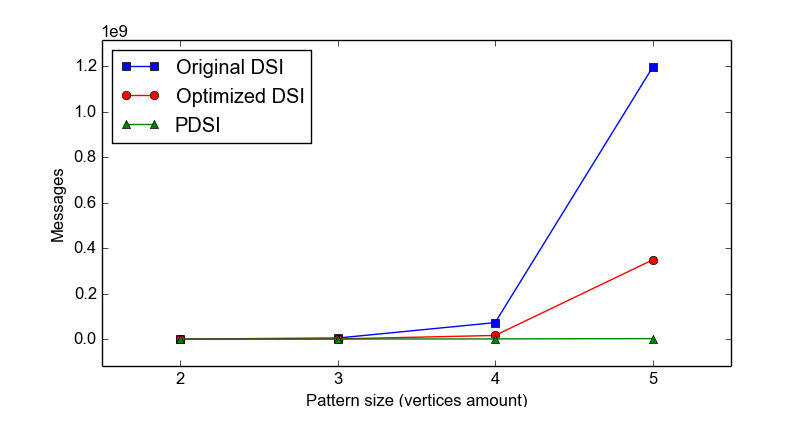
\includegraphics[width=\textwidth]{messages-Ps.png}
    \caption{Total message amount of DSI, optimized DSI and PDSI with patterns of different sizes}
    \label{fig:messages-P}
  \end{center}
\end{figure}

Another property of the algorithms to evaluate is the maximum supersteps. Table~\ref{tab:iterations} shows the how many supersteps that each algorithm has executed for different pattern sizes. All of them have the same amount of supersteps as the theoretical upper bound, which is $2 + k*(k-1)/2$ (our implementation uses one additional superstep to gather the neighboring vertices IDs). As the patterns are small and simple, it is possible to traverse the longest route in the data graph.

\newcolumntype{C}{>{\centering\arraybackslash}p{5em}}
\begin{table}[H]
  \begin{center}
    \begin{tabular}{|C|C|C|C|C|}
    \hline
    Pattern Size & DSI & Optimized DSI & PDSI & Upper Bound \\ \hline 
    2 & 3 & 3 & 3 & 3 \\ \hline
    3 & 5 & 5 & 5 & 5 \\ \hline
    4 & 8 & 8 & 8 & 8 \\ \hline
    5 & 12 & 12 & 12 & 12 \\ \hline
    \end{tabular}
    \caption{Supersteps of DSI, optimized DSI and PDSI with patterns of different sizes}
    \label{tab:iterations}
  \end{center}
\end{table}

We also evaluate the duplication of the found subgraphs. Figure~\ref{fig:repetitions-P} shows that subgraph duplication factor of the algorithms, which is the result that total found subgraphs amount is divided by the number of identical subgraphs. The duplication factor increases intensively as the pattern size grows. While DSI and optimized DSI have found the same number of identical subgraphs, DSI duplicates about 6000 times and optimized DSI duplicates about 1600 times when the pattern size is 5. It is mainly because the routes to find isomorphic subgraphs become more variant when the pattern size grows. PDSI does not guarantee that all subgraphs are found, but the duplication factor is relatively low.

\begin{figure}[H]
  \begin{center}
    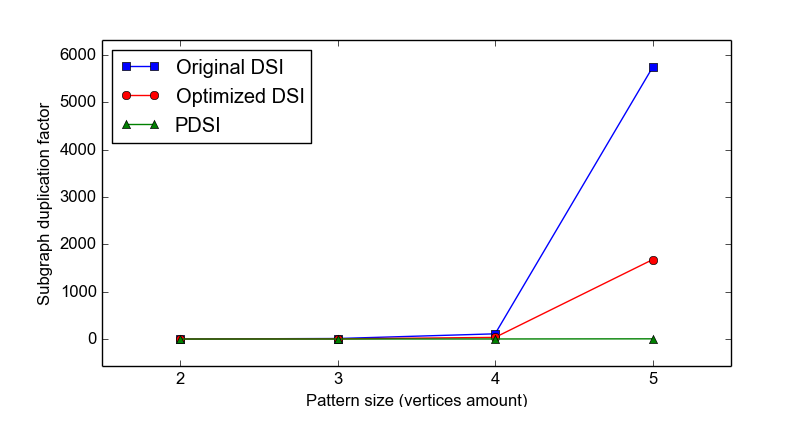
\includegraphics[width=\textwidth]{repetitions-Ps.png}
    \caption{Subgraph duplication factor of DSI, optimized DSI and PDSI with patterns of different sizes}
    \label{fig:repetitions-P}
  \end{center}
\end{figure}

As PDSI does not guarantee neither the existence nor the completeness of isomorphic subgraphs, we are interested in how many isomorphic subgraphs can be found by PDSI. Figure~\ref{fig:foundproportion-P} shows the percentage of the found identical subgraphs by PDSI. With the proportion 0.3, PDSI can find a large part of identical subgraphs, and has very low runtime and subgraph duplication factor.

\begin{figure}[H]
  \begin{center}
    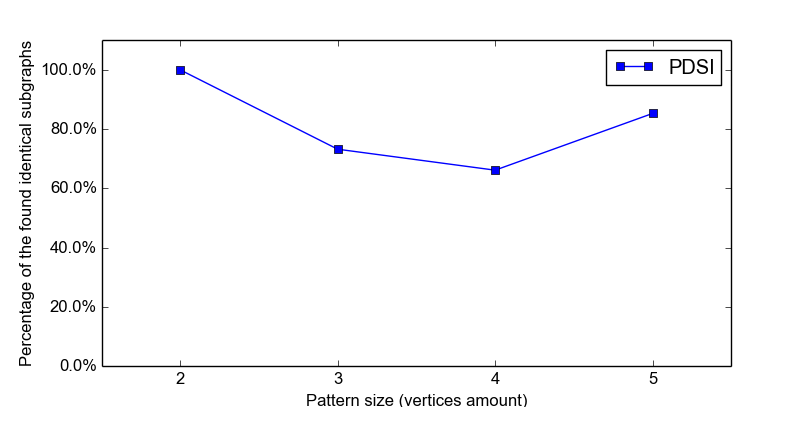
\includegraphics[width=\textwidth]{foundproportion-Ps.png}
    \caption{Percentage of the found identical subgraphs by PDSI with patterns of different sizes}
    \label{fig:foundproportion-P}
  \end{center}
\end{figure}

\subsection{Impact of Data Graph Size}

We evaluate the original DSI, optimized DSI and PDSI with data graphs of different sizes to study the properties of the algorithms. The data graphs we used are the subsets of ego-Twitter. The data graphs are increased by randomly adding vertices and their associating edges, which size varies from 42771 vertices to 81306 vertices. The pattern size is 3, and the number of machines is 11. For optimized DSI and PDSI, the initial vertex is randomly chosen. For PDSI, the parameter proportion is 0.1.

Figure~\ref{fig:runtime-G} shows that the runtime increases nonlinearly as the size of the data graph grows. The runtime behaviour also shows the computational complexity of the algorithms. The optimized DSI reduces the complexity and only takes about one third runtime as DSI needs. As PDSI uses the proportion to reduce the complexity, which also introduces non-deterministic factor to the runtime. Figure~\ref{fig:messages-G} shows that total message amount generated during the execution. The runtime increases with the same rate as the message amount grows.

\begin{figure}[H]
  \begin{center}
    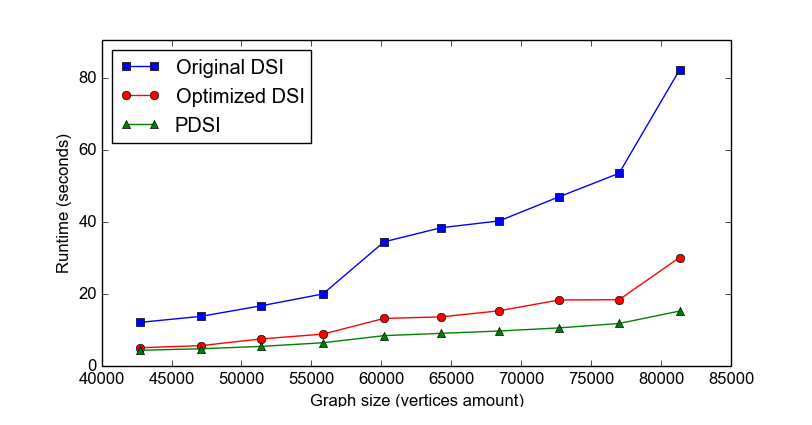
\includegraphics[width=\textwidth]{runtime-G.png}
    \caption{Runtime of DSI, optimized DSI and PDSI with data graphs of different sizes}
    \label{fig:runtime-G}
  \end{center}
\end{figure}

\begin{figure}[H]
  \begin{center}
    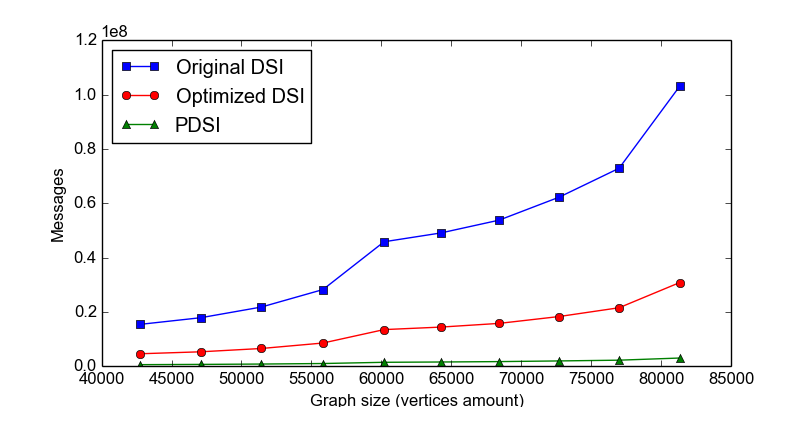
\includegraphics[width=\textwidth]{messages-Gs.png}
    \caption{Total message amount of DSI, optimized DSI and PDSI with data graphs of different sizes}
    \label{fig:messages-G}
  \end{center}
\end{figure}

\subsection{Impact of Machines}

We evaluate the runtime of original DSI, optimized DSI and PDSI with different number of machines to study the performance and scalability. The number of machines is increased from 2 to 11. The data graph is ego-Twitter and the pattern size is 3. For optimized DSI and PDSI, the initial vertex is randomly chosen. For PDSI, the parameter proportion is 0.1.

We can observe in Figure~\ref{fig:runtime-M} that PowerGraph scales very well with the three algorithms for subgraph isomorphism. With two optimization strategies, the optimized DSI only takes about one third runtime as DSI needs. PDSI with proportion 0.1 takes two third runtime as optimized DSI takes. The main reason is that execution with a pattern of size 3 do not have so many iterations. In addition, randomly selecting a proportion of messages in the gather phase introduces latency.

\begin{figure}[H]
  \begin{center}
    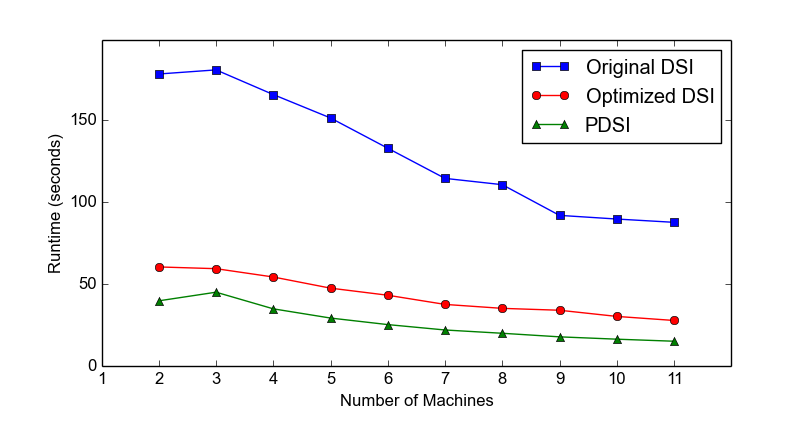
\includegraphics[width=\textwidth]{runtime-M.png}
    \caption{Runtime of DSI, optimized DSI and PDSI with different numbers of machines}
    \label{fig:runtime-M}
  \end{center}
\end{figure}

\subsection{Impact of the Proportion in PDSI}

The experiments were conducted by increasing the parameter proportion from 0.1 to 1. The data graph is ego-Twitter, the pattern size is 3, and the number of machines is 11. The initial vertex is randomly chosen. In Figure~\ref{fig:runtime-PP} we can see that the runtime can be well controlled by adopting different proportions. The runtime is almost linear to the proportion.

\begin{figure}[H]
  \begin{center}
    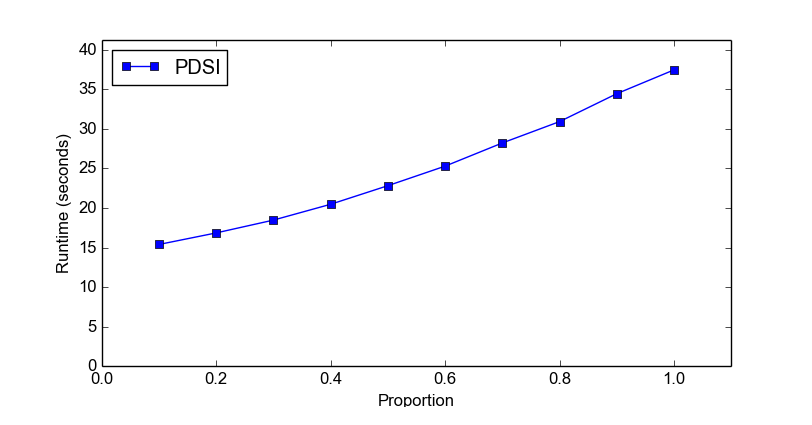
\includegraphics[width=\textwidth]{runtime-PP.png}
    \caption{Runtime of PDSI with different proportions}
    \label{fig:runtime-PP}
  \end{center}
\end{figure}

We show the duplication factor of PDSI with different proportions in Figure~\ref{fig:repetitions-PP}. The duplication factor increases with the proportion. High proportion leads to high messages quantity followed by high duplication factor.

\begin{figure}[H]
  \begin{center}
    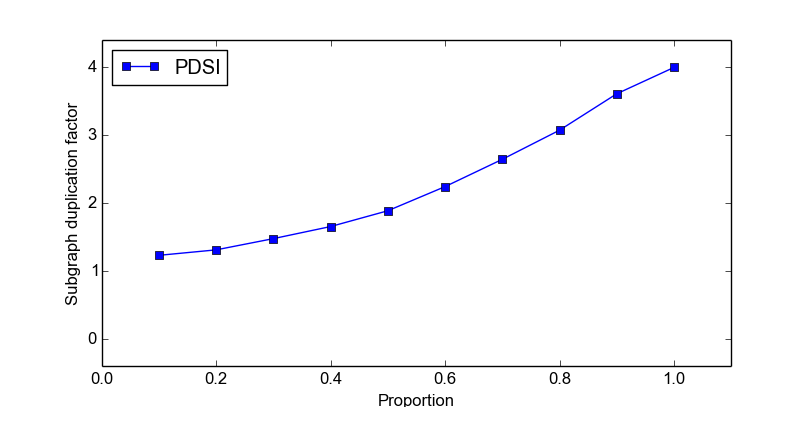
\includegraphics[width=\textwidth]{repetitions-PPs.png}
    \caption{Subgraph duplication factor of PDSI with different proportions}
    \label{fig:repetitions-PP}
  \end{center}
\end{figure}

Figure~\ref{fig:foundproportion-PP} shows that the percentage of found identical subgraphs increases with the proportion. We can see that PDSI can find more than 80\% of the subgraphs just with the proportion 0.5.

\begin{figure}[H]
  \begin{center}
    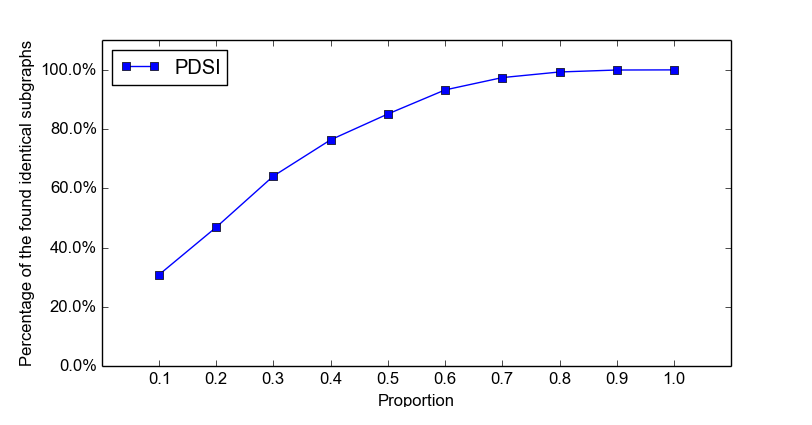
\includegraphics[width=\textwidth]{foundproportion-PPs.png}
    \caption{Percentage of the found identical subgraphs by PDSI with different proportions}
    \label{fig:foundproportion-PP}
  \end{center}
\end{figure}

\section{Evaluation of the Communication Costs for Synchronization}
\label{sec: evaluation-heterogeneity}

In the really world, the communication costs for synchronization are often heterogeneous. Therefore, we evaluate the vertex synchronization costs of the optimized DSI and geospatial simulation. Figure~\ref{fig:heterogeneity-ODSI} shows the number of vertices against the vertex synchronization costs in optimized DSI. The most vertices have the vertex synchronization costs below 200 kilobytes, while a few vertices have much more communication.

\begin{figure}[H]
  \begin{center}
    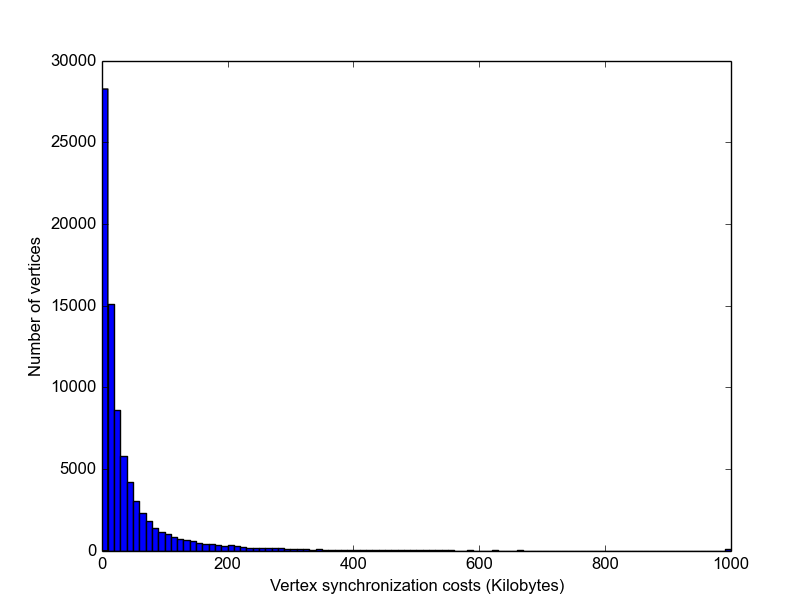
\includegraphics[width=\textwidth]{heterogeneity-ODSI.png}
    \caption{Vertex synchronization costs of optimized DSI on ego-Twitter graph with a 3-vertices pattern}
    \label{fig:heterogeneity-ODSI}
  \end{center}
\end{figure}

To evaluate geospatial simulation, we used the GPS trajectory dataset collected in Geolife project\footnote{http://research.microsoft.com/en-us/projects/geolife/default.aspx}. These trajectories were recorded by different GPS devices, and have a variety of sampling rates. Over 90\% of the trajectories were logged in a dense representation, e.g. every 1-5 seconds or every 5-10 meters per point. Although this dataset is wildly distributed in many cities, a subset of the data is used to simulate the agents mobility within Beijing, which contains in total 98 agents. The movements of agents are simulated in the time span of one day. The simulation time interval is 10 seconds. The area is divided into 10000 grids, each of which connects to its Moore neighborhood. Figure~\ref{fig:heterogeneity-ABCA} shows that the most vertices have very low communication costs for synchronization. This is mainly because that there are some hotspots in which the agents move.

\begin{figure}[H]
  \begin{center}
    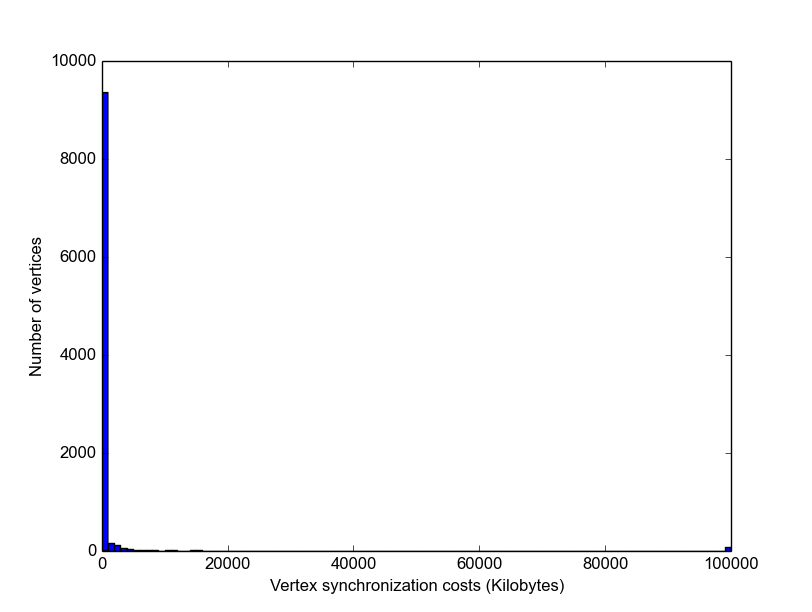
\includegraphics[width=\textwidth]{heterogeneity-ABCA.png}
    \caption{Vertex synchronization costs of geospatial simulation}
    \label{fig:heterogeneity-ABCA}
  \end{center}
\end{figure}


\section{Evaluation on GrapH}

GrapH is a framework prototype under developing in the University of Stuttgart, which takes the vertex synchronization costs into account to optimize graph partitioning. It loads graph by a static edge mapping algorithm and uses an adaptive partitioning strategy to migrate edges dynamically. 
%User can specify a parameter to control how many supersteps the adaptive partitioning to be performed, which lets user to balance the migration overhead in time.\textbf{TODO} 
Another feature of GrapH is that it keeps the graph in memory so that it can continuously perform different computation on the same graph with loading the graph only once. We evaluate the optimized DSI and geospatial simulation on GrapH to study the communication improvement by GrapH.

We performed optimized DSI on the ego-Twitter graph. We continuously executed 30 simple pattern queries, each of which consists of 2 or 3 vertices. We compare two executions with and without adaptive partitioning based on the PowerGraph pre-partitioned graph. The Figure~\ref{fig:si-pre-n10} shows that the accumulative communication including the migration costs between machines is reduced more than 20\% when using adaptive partitioning. As optimized DSI has complex computation and large data size, the costs for migrating edges are relatively low and negligible.

\begin{figure}[H]
  \begin{center}
    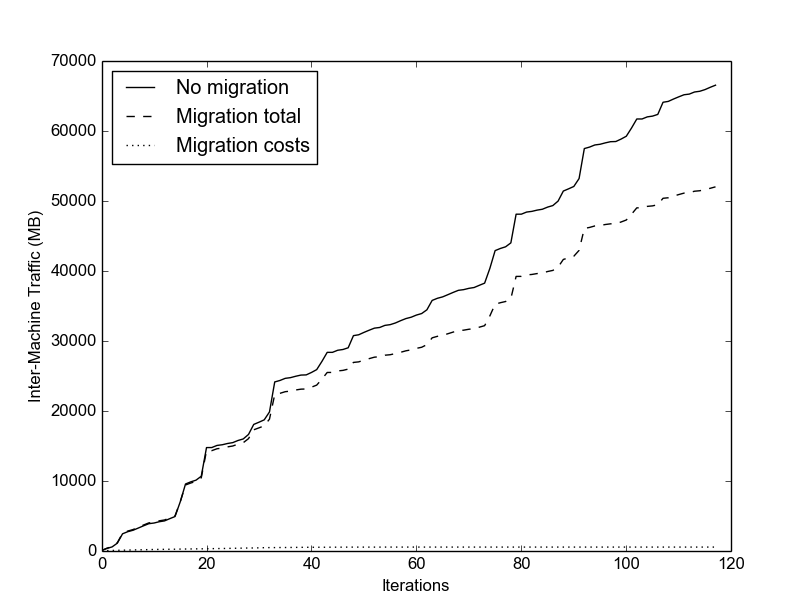
\includegraphics[width=\textwidth]{si-pre-n10.png}
    \caption{Accumulative inter-machine traffic of optimized DSI}
    \label{fig:si-pre-n10}
  \end{center}
\end{figure}

Figure~\ref{fig:si-pre-n10-c} shows the inter-machine traffic of each superstep. With the migration, the current inter-machine traffic is reduced gradually, and at the end the current traffic has been reduced about 30\%.

\begin{figure}[H]
  \begin{center}
    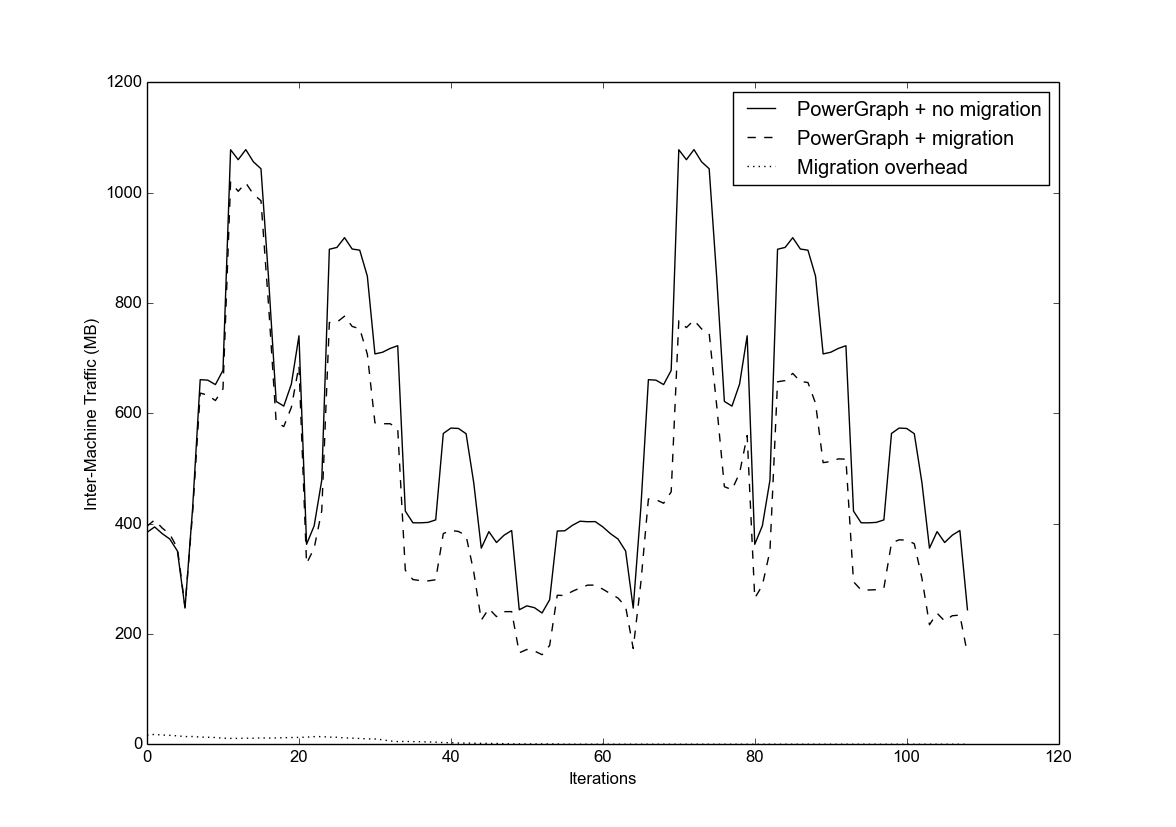
\includegraphics[width=\textwidth]{si-pre-n10-c.png}
    \caption{Current inter-machine traffic of optimized DSI}
    \label{fig:si-pre-n10-c}
  \end{center}
\end{figure}

In the evaluation of optimized DSI on GrapH, the adaptive partitioning strategy increases the latency slightly, which takes 5109 seconds, compared with 4904 seconds of the execution without adaptive partitioning.

We also performed the geospatial simulation with the same setting as we did in \ref{sec: evaluation-heterogeneity} except that the time interval is 1200 seconds. The PowerGraph pre-partitioned graph was loaded to GrapH and executed with and without adaptive partitioning. The latency is also increased by adaptive partitioning, which is 927 seconds, compared with 664 seconds of the execution without adaptive partitioning. The Figure~\ref{fig:ca-pre-n10} shows that the accumulative communication including the migration costs between machines is reduced more than 20\% by the adaptive repartition.

\begin{figure}[H]
  \begin{center}
    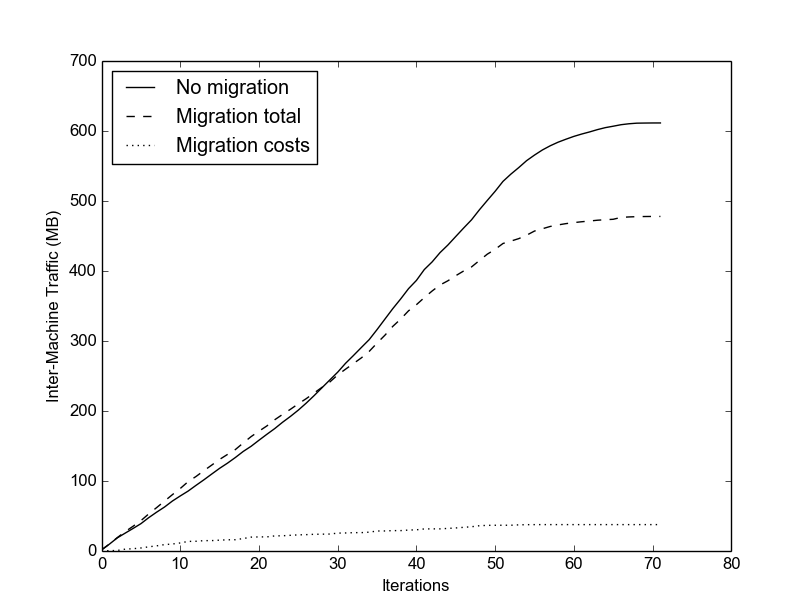
\includegraphics[width=\textwidth]{ca-pre-n10.png}
    \caption{Accumulative inter-machine traffic of geospatial simulation}
    \label{fig:ca-pre-n10}
  \end{center}
\end{figure}

Figure~\ref{fig:si-pre-n10-c} shows the inter-machine traffic of each superstep. At the beginning of migration, the current inter-machine traffic of the one with adaptive partitioning is a little bit higher than the one without adaptive partitioning due to the migration costs. However, the current inter-machine traffic has been reduced by the migration about 50\% at the end.

\begin{figure}[H]
  \begin{center}
    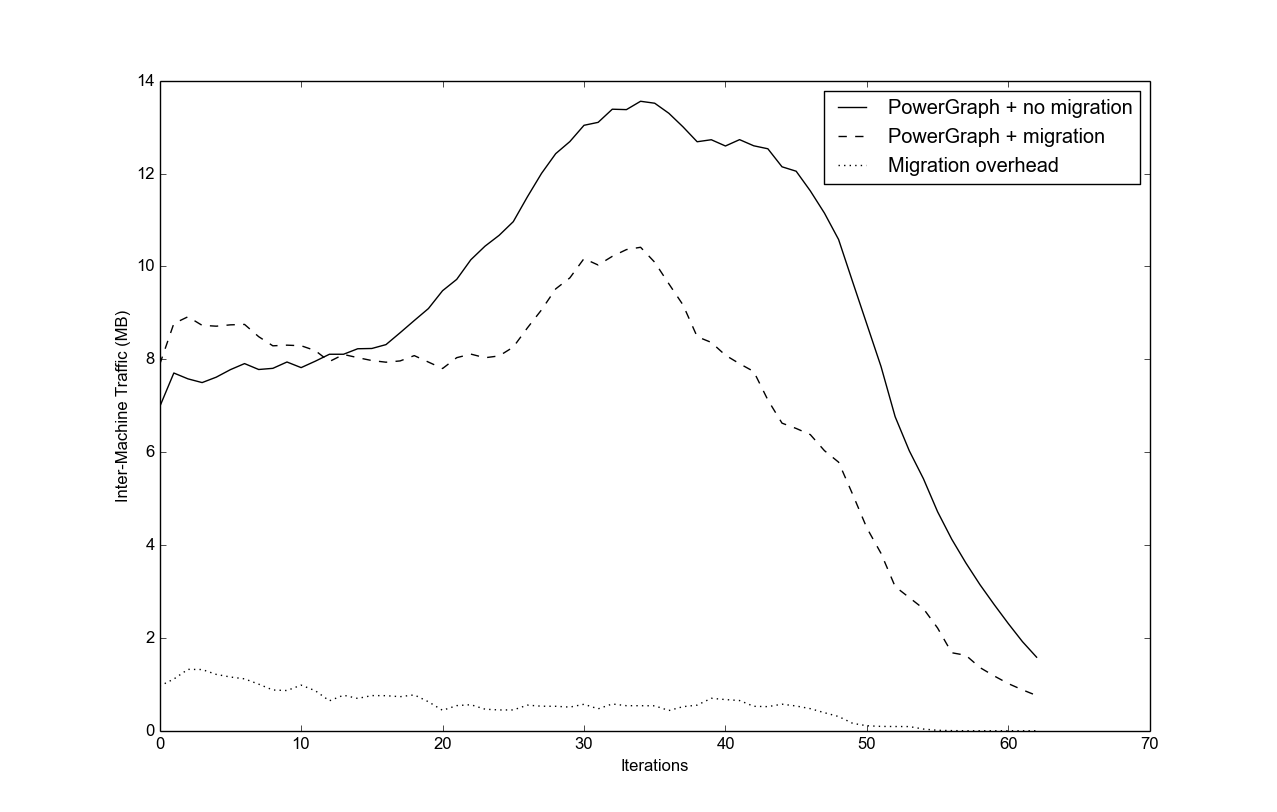
\includegraphics[width=\textwidth]{ca-pre-n10-c.png}
    \caption{Current inter-machine traffic of geospatial simulation}
    \label{fig:ca-pre-n10-c}
  \end{center}
\end{figure}
\chapter{Conclusion and Outlook}\label{chap:c6}

The emergence of graph processing frameworks empowered us to efficiently solve problems of large graphs. In this thesis, we designed novel algorithms on graph processing frameworks to solve two typical problems, subgraph isomorphism and geospatial simulation. 

The subgraph isomorphism is the core problem of graph pattern matching, however no existing algorithm was designed for executing on a graph processing framework. We innovatively designed an algorithm DSI and its variants, which fit to the GAS programming model. The properties of the algorithms, such as computational complexity and etc. have been analysed. DSI, optimized DSI and PDSI were implemented on PowerGraph and GrapH. The evaluation shows that the runtime mainly depends on the message amount. The message amount increases when the pattern size or the data graph size grows. However, the pattern size is dominant, because the message amount is exponential to the total supersteps, which upper bound depends on the size of the pattern. As the messages boost, the resources might be exhausted. The isomorphic subgraphs found by the algorithms are highly duplicated, specially for large patterns. The reason is that the routes for finding isomorphic subgraphs become variant when the pattern size increases. Parallelism by increasing machines can reduce the runtime. The results also show that the optimized DSI takes on average only one third of execution time as DSI needs. PDSI can remarkably reduce the runtime with a low proportion, and still be able to find a relative reasonable quantity of the isomorphic subgraphs. High proportion creates high message amount, which leads to both high duplication factor and more found identical subgraphs. Choosing a reasonable proportion depends on many factors, such as resource availability and searching requirements.

Although these algorithms can solve the problem of subgraph isomorphism in a distributed environment, the performance is limited by the increase of messages. Even with the optimized DSI, the runtime is still very long for large patterns. So DSI needs further optimization. Pre-knowledge of the data graph and analysing the pattern could be helpful to choose an optimal initial vertex. Techniques such as graph invariants that restrict the matching criteria can further reduce the message quantity.

Geospatial simulation is a popular research topic. As the scale of the simulation becomes larger, different parallel distributed computing systems are designed and used for geospatial simulation. We argue that graph processing framework is a good option, and we innovatively used GAS programming paradigm to express the Agent-Based Cellular Automata model, which is able to represent both spatio-temporal and agent dynamics. Since our algorithm for geospatial simulation only simulates simple moving behaviors, simulating complicated behaviors and systems on graph processing frameworks is still open.

%Parallelism for geospatial simulation enables processing large and complex system. Geospatial simulation using Agent-Based Cellular Automata is implemented in the GAS programming model on both PowerGraph and a prototypical framework. The evaluation results show that ...

The evaluation of both subgraph isomorphism and geospatial simulation shows the vertex synchronization costs are heterogeneous: only a few vertices dominate the most communication costs for synchronization. Modern graph processing frameworks like PowerGraph partition the graph with vertex-cut to achieve workload balance and communication balance, which shows a good result on the real world graphs of power-law degree distribution. However, they fail to consider the heterogeneity of the vertex synchronization costs. GrapH covers this gap by introducing adaptive partitioning to minimize communication. Based on the PowerGraph pre-partitioned graph, GrapH reduces communication by edge migration and only slightly increases the latency. GrapH outperforms PowerGraph with respect to overall communication, which are reduced more than 20\% in our evaluation.

As processing large graphs becomes more and more popular, the improvement of frameworks performance will bring more benefits. For instance, further work may be to refine the adaptive partitioning strategy and consider the network heterogeneity.

%\input{content/zusammenfassung_und_ausblick}
%
%
%\renewcommand{\appendixtocname}{Anhang}
%\renewcommand{\appendixname}{Anhang}
%\renewcommand{\appendixpagename}{Anhang}
\appendix
%\input{content/anhang}
%\printindex
%\bibliographystyle{alphadin}
\ifdeutsch
\bibliographystyle{bibliography/IAASde} %f"ur deutsche Texte
\else
\bibliographystyle{bibliography/IAAS} %f"ur englische Texte
\fi
\bibliography{bibliography/bibliography}
\ifdeutsch
Alle URLs wurden zuletzt am 17.\,03.\,2008 geprüft.
\else
All links were last followed on December 21, 2008.
\fi

\backmatter 
\pagestyle{empty}
\renewcommand*{\chapterpagestyle}{empty}
\Versicherung
\end{document}
